\documentclass[conference]{IEEEtran}
\usepackage[english]{babel}
\usepackage{geometry}
\usepackage{amsmath}
\usepackage{amsthm}
\usepackage{graphicx}
\usepackage{caption}
\usepackage[utf8]{inputenc}


%%%%%%%% SUB-FIGURE PACKAGE
\usepackage{subcaption}

%%%%%%%% MULTI-COLUMNS PACKAGE
\usepackage{multicol}

%%%%%%%% PERSONAL COMMANDS
\usepackage{amssymb}

%%%% Important sets
\renewcommand{\O}{\mathbb{O}}
\newcommand{\N}{\mathbb{N}}
\newcommand{\Z}{{\mathbb{Z}}}
\newcommand{\Q}{{\mathbb{Q}}}
\newcommand{\R}{{\mathbb{R}}}

%%%% Usual operations
\newcommand{\pow}[2]{#1^{#2}}
\newcommand{\expp}[1]{e^{#1}}
\newcommand{\fst}{\mathrm{fst}}
\newcommand{\snd}{\mathrm{snd}}

%%%% Lambda Calculus
\newcommand{\dneq}{\,\, \# \,\,}
\newcommand{\prm}[1]{\mathrm{\mathbf{#1}}}
\renewcommand{\S}{\prm{S}}
\newcommand{\I}{\prm{I}}
\newcommand{\K}{\prm{K}}
\newcommand{\ch}[1]{\ulcorner #1 \urcorner}

%%%% Ordinal Lambda Calculus
\newcommand{\ordAlph}{\Sigma_{\text{Ord}}}
\newcommand{\termOrd}{\text{Term}_\text{Ord}}
\newcommand{\fl}{\mathrm{fl}}
\newcommand{\sk}{\mathrm{sk}}

%% Superscript to the left
% https://latex.org/forum/viewtopic.php?t=455
\usepackage{tensor}
\newcommand{\app}[3]{\tensor*[^{#1}]{\left(#2, #3\right)}{}}

%%%% Make optional parameter
% https://bit.ly/3jVGRwQ
\usepackage{xparse}

%%%% Statistics
\NewDocumentCommand{\E}{o m}{
  \IfNoValueTF{#1}
  {\mathbb{E}\left[#2\right]}
  {\mathbb{E}^{#1}\left[ #2\right]}
}
\NewDocumentCommand{\V}{o m}{
  \IfNoValueTF{#1}
  {\mathrm{Var}\left[#2\right]}
  {\mathrm{Var}^{#1}\left[ #2\right]}
}
\RenewDocumentCommand{\P}{o o m}{
  \IfNoValueTF{#1}
  {\IfNoValueTF{#2}
    {\mathrm{P}\left(#3\right)}
    {\mathrm{P}^{#2}\left(#3\right)}}
  {\IfNoValueTF{#2}
    {\mathrm{P}_{#1}\left(#3\right)}
    {\mathrm{P}_{#1}^{#2} \left(#3\right)}}
}

%%%% Lambda Calculus
\NewDocumentCommand{\cx}{o}{
  \IfNoValueTF{#1}
  {\left[\quad\right]}
  {\left[\, #1 \,\right]}
}

%%%% Create absolute value function
% https://bit.ly/33Rkq6H
\usepackage{mathtools}
\DeclarePairedDelimiter\abs{\lvert}{\rvert}%
\DeclarePairedDelimiter\norm{\lVert}{\rVert}%
\makeatletter
\let\oldabs\abs
\def\abs{\@ifstar{\oldabs}{\oldabs*}}
%
\let\oldnorm\norm
\def\norm{\@ifstar{\oldnorm}{\oldnorm*}}
\makeatother

%%%%%%%% LOGIC TREES
\usepackage{prftree}

%%%%%%%% SPLIT EQUATIONS
% https://bit.ly/33P1OUM
\allowdisplaybreaks

%%%%%%%% FLOAT SPECIFIER
% https://bit.ly/30Wi4BC
\usepackage{float}

%%%%%%%% TO USE SHORT COMMANDS FOR VECTOR LINES
\usepackage{esvect}

%%%%%%%% DIFFERENT FONTS FOR MATH
\usepackage{mathrsfs}

%%%%%%%% FOOTNOTE STUFF
\renewcommand{\thefootnote}{\fnsymbol{footnote}}



%%%%%%%% MARGIN
\geometry{verbose, letterpaper, tmargin=3cm,
  bmargin=3cm,lmargin=2.5cm,rmargin=2.5cm}

%%%%%%%% PARAGRAPH SETTINGS
% https://bit.ly/36WrtN4
\setlength\parindent{0pt}

% https://bit.ly/371dvto
\setlength{\parskip}{5pt}

%%%%%%%% HYPERREF PACKAGE
\usepackage{hyperref}
\hypersetup{linkcolor=blue}
\hypersetup{citecolor=blue}
\hypersetup{urlcolor=blue}
\hypersetup{colorlinks=true}


%%%%%%%% BIB-LATEX STUFF
\usepackage[style=ieee,
            bibstyle=ieee,
            citestyle=ieee,
            hyperref=true,
            backend=biber]{biblatex}
\addbibresource{ref.bib} %Put relative path to ref

%%%%%%%% DEFINITION AND THEOREM DEFINITIONS
\theoremstyle{definition}
\newtheorem{definition}{Definition}[section]

\theoremstyle{remark}
\newtheorem{remark}{Remark}

\theoremstyle{remark}
\newtheorem{question}{Question}

\newtheorem{theorem}{Theorem}[section]


%%%%%%%% CODE RENDERING !!! UNCOMMENT IF NEEDED !!!
% Compile with flag -shell-escape
%\usepackage{minted}

%%%%%%%% START DOCUMENT
\title{Supervised Learning for Psychological Attention to High School Students}

\author{\IEEEauthorblockN{Juan Sebastián Cárdenas-Rodríguez}
  \IEEEauthorblockA{\textit{Department of Mathematical Sciences} \\
    \textit{EAFIT University}\\
    Medellín, Colombia \\
    jscardenar@eafit.edu.co} \and \IEEEauthorblockN{David Plazas}
  \IEEEauthorblockA{\textit{Department of Mathematical Sciences} \\
    \textit{EAFIT University}\\
    Medellín, Colombia \\
    dplazas@eafit.edu.co} }


\begin{document}
\maketitle

%%%%%%%%%%%%%%%%%%%%%%%%%%%%%
\begin{abstract}
  Hello.
\end{abstract}

\begin{IEEEkeywords}
  Nice.
\end{IEEEkeywords}
%%%%%%%%%%%%%%%%%%%%%%%%%%%%%

\textit{Note}: All the code and the latex file can be found in
\href{https://github.com/juanscr/ai-works}{the GitHub repository}.

\section{Introduction}

Mental health is crucially important for every human being and has become one of
the most important issues surrounding human health. According to the World
Health Organization (WHO)\footnote{WHO's \href{https://bit.ly/34l2v94}{2001
    report.}} report of 2001, mental disorders can affect 25\% of the
population, therefore, suggesting the ongoing trend of people suffering from
lack of mental health. Additionally, with the recent events caused by the
COVID-19 pandemic, mental issues have risen as consequence of lockdowns all
around the globe, as have been proved by recent studies
\parencite{rossi2020,xiong2020}.

Furthermore, mental health is more important to monitor in adolescents and kids
as this group is in the process of developing their mental structure and
character. In this manner, as they continue creating their view about the world
they must be surrounded by a healthy environment that promotes healthy habits
and relationships with their surroundings.

As a result, schools and parents have an important responsibility to the
students of creating this environment and wisely handling mental health issues.
However, high schools do not always know how to handle or detect cases of mental
health issues. Additionally, technology has led to targeted harassing becoming
more popular over time, therefore, complicating the probability of detecting
these cases.

Some of the most common and important mental health issues are anxiety,
depression, and hyperkinetic disorder. According to \textcite{schulte2016},
around 10\% to 20\% of children suffer from hyperkinetic disorder. Additionally,
school teachers just assume this disorder is a cause of undisciplined students
and can take the hyperkinetic student to a depressive state. These three mental
disorders can leave severe damage to a kid and can lead them to suicide.

Hence, it is of the utmost importance to quickly and efficiently detect students
that might be having a mental health issue to immediately start a process with
him/her. Furthermore, this detection has to be done with measurable variables
that can be easily obtained from questionnaires or school data.

The present work is oriented to the application of supervised learning
techniques (decision trees, support vector machines and neural networks) for
classifying the data from the survey, aiming for the construction of a model to
detect individuals with mental health issues. Recent developments and the
increasing popularity of supervised techniques has contributed to their
application in different areas, among them, mental health.

The novel work by \textcite{thieme2020} makes and excellent literature review of
Machine Learning (ML) in mental health, including the current state-of-the-art
and formulates new strategies for integrating human-oriented research with
multi-disciplinary. They also conclude that ML applied in mental health is
``still in its infancy'' given the complexity and difficulties of constructing
robust models for clinically reliable outputs.

Additionally, the work presented by \textcite{shatte2019} is also a complete
compendium of recent ML applications in mental health, including the usage of
Support Vector Machines (SVMs), Decision Trees (DTs), Neural Networks (NN) and
beyond. This paper includes a systematic review of over three hundred papers and
it concludes that these techniques have brought benefits across the areas of
diagnosis, treatment, research and clinical administration.

Finally, another overview of applications of Artificial Intelligence (AI) for
Mental Illnesses is the research published by \textcite{graham2019}, where the
authors reviewed 28 research papers which include modern methodologies (and
technologies) for predicting or classifying psychological illnesses such as
depression, schizophrenia or suicidal behavior. The study discusses how the
application of AI techniques supports the clinical practice while considering
its limitations, it also presents some ethical implications and states which
areas need further development.

This document is organized as follows: Section \ref{sec:meth} shows the general
methodology used in this work, moreover Section \ref{sec:res} shows the obtained
results over the data and slight modifications, finally Section \ref{sec:conc}
concludes this work and sets pillars for future works.

\section{Methodology}\label{sec:meth}
All the code developed for this work was implemented in Julia 1.5.3. and
can be found in the authors'
\href{https://github.com/juanscr/ai-works}{GitHub repository}, although the
plots were generated using Python 3.8.6.

\subsection{Survey}
The used survey for extracting data was initially designed in the developing a
Fuzzy Inference System, but the data was labeled according to unsupervised
clustering techniques, obtaining 2 clusters through the subtractive algorithm
\parencite{chiu1994} and then sharpened using Fuzzy-C-Means
\parencite{dunn1973}. The data has 6 variables and 113 observations. This
dataset was divided with the standard $60-20-20$ rule, creating a training
dataset with $60\%$ of the complete data, a validation set with $20\%$ and a
test set with $20\%$ as well. All data was normalized by dividing each dimension
by its maximum (in absolute value), casting the data into the [-1,1] hypercube.

Remark: the dataset includes both inputs (first three variables) and outputs
(last three variables) of the Fuzzy Inference System. This will be later useful
to organize relationships in the variables for more intuitive plots.

\subsection{Support Vector Machines}
\textcite{burges1998} published an excellent reference for the theoretical
background on SVMs with different kernels and explains the formulation of the
optimization problem. The SVMs were used directly from Scikit-Learn
\parencite{scikit-learn, sklearn_api} using
\href{https://bit.ly/3lDHADX}{Julia's API}. The SVMs were trained using three
different kernels: linear, polynomial and RBF (radial base function).

Given that the sample size is fixed, the analysis for the ``Probably
Approximately Correct'' (PAC) learning was not straight-forward, as the
classifier's maximum permitted error $\epsilon$ was estimated from the classic
formulae, rather than calculating the adequate sample size for a given $\delta$.

The PAC learning here applied is based on the ideas presented in
\parencite{kubat2017}. Let $N$ be number of samples in the training set,
$\epsilon$ is the classifier maximum permitted error rate, $\delta$ is the
probability that a classifier with error rate greater than $\epsilon$ is
\text{error-free} on the training set, $m$ be the dimension of each training
pattern, and let $VC$ be the Vapnik-Chervonenkis dimension of the given
classifier. Hence, for learning in continuous domains, the lower bound for $N$
is

\begin{equation}
  N\geq \max\left\{ \dfrac{4}{\epsilon}\ln\left(\dfrac{2}{\delta}\right),
    \dfrac{8\mathrm{VC}}{\epsilon}\ln\left(\dfrac{13}{\epsilon}\right) \right\}.
\end{equation}

It is clear that solving for $\epsilon$ is non-trivial for given values of
$\delta$, $N$ and $\mathrm{VC}$; thus, an optimization approach was used to
estimate $\epsilon$ for the input values, solving the nonlinear optimization
problem

\begin{equation}
  \begin{split}
    \min_{\epsilon\in\mathbb{R}_+}\ &J=\,\epsilon^2\\
    \mathrm{s.t.}\ &\dfrac{4}{\epsilon}\ln\left(\dfrac{2}{\delta} \right)\leq N\\
    \quad&\dfrac{8\mathrm{VC}}{\epsilon}\ln\left(\dfrac{13}{\epsilon}\right)\leq N.
  \end{split}
\end{equation}

The problem was initially constrained to $\epsilon\in[0,1]$, but it had not
feasible solution for the size of the training set, yielding values of
$\epsilon$ greater than 1. Instead, the constrained was removed and a
sensitivity analysis was made for the training set size, varying the latter to
find a suitable value for $\epsilon$. The size of training set was varied in
$(0.8N, 10N)$ for each kernel SVM and the estimated $\epsilon$ are presented in
Fig. \ref{fig:error-SVM}, with a fixed $\delta$. Note that $\mathrm{VC}=7$ for
the linear SVM, since $m=6$, and $\mathrm{VC}=84$ for the polynomial SVM, since
cubic polynomials were selected; furthermore, the VC dimension for the RBF SVM
is infinite and this case was not included (see \parencite{burges1998}).

Note that $\epsilon$ in the linear SVM enters the feasible value for training
sets above 150 samples and stabilizing around $\epsilon=0.3$ for large training
set samples value. In contrast, $\epsilon$ for the polynomial SVM never reaches
a suitable value below 1, indicating that this classifier requires more than 600
samples in the training set to satisfy the PAC learning.

\begin{figure}
  \centering
  \begin{subfigure}[b]{0.45\textwidth}
    \centering 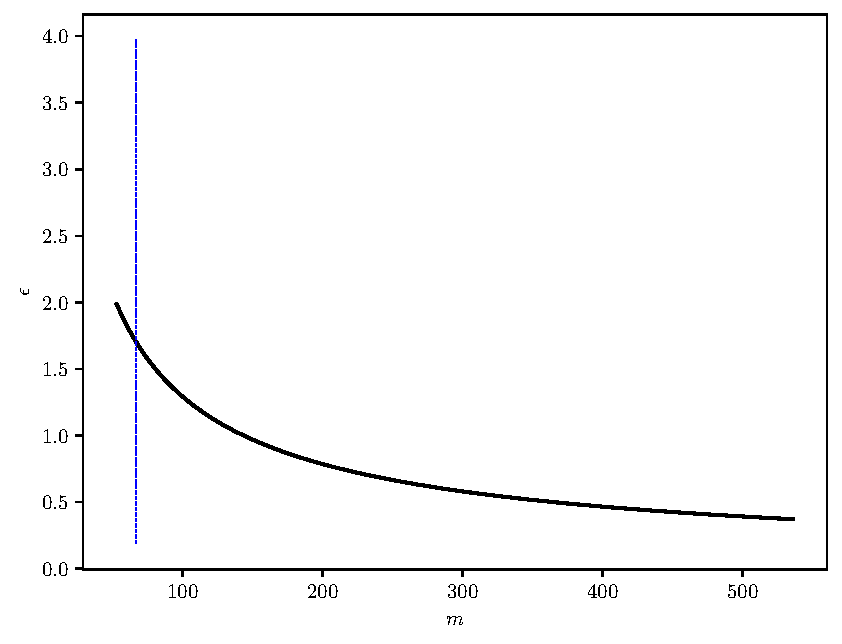
\includegraphics[width=\textwidth]{figs/svm-linear-error.pdf}
    \caption{Linear SVM.}
  \end{subfigure}
  \begin{subfigure}[b]{0.45\textwidth}
    \centering 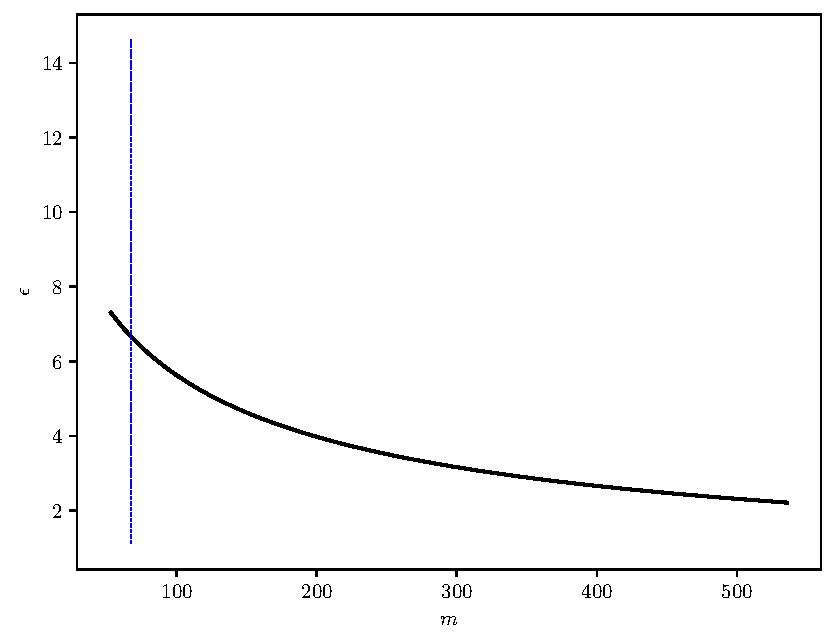
\includegraphics[width=\textwidth]{figs/svm-poly-error.pdf}
    \caption{Polynomial SVM}
  \end{subfigure}
  \caption{Estimated $\epsilon$ for different training set sizes.}
  \label{fig:error-SVM}
\end{figure}

Furthermore, it is important to notice that the dataset is 6-dimensional, which
clearly brings problems for visualizing the learning machines' outputs and
decision boundaries. In this paper, the decision functions of the fitted
learning machines will be presented using contour plots of the projected data.
This process will better described: each 6-dimensional pattern generates an
output whenever it is evaluated in the fitted model. The idea is to generate an
equally-spaced grid in $[-1,1]^6$ and evaluate each point on this model, in
order to plot the contour of the shattering function. The main issue is that a
direct projection into a 2-dimensional space of each point on the grid is not
necessarily a function, since several points can have the same projection, but
different values of the shattering function. In order to address this issue, the
mean of the points that mapped into the same projection is taken, giving an
proxy of the general behavior in high dimensions. This ``mean'' projection
contour plots also include the projection of the training data points into the
same coordinates and scattered with the real labels, giving an idea of the
classification performance in high dimensions. Remark: as stated, the survey
data also includes the outputs of the Fuzzy Inference System; thus, the contour
plots are presented only for relating first input with the first input, second
with the second output and so on. This was done aiming at two objectives:
keeping a reasonable number of plots in the document, and giving a more
intuitive interpretation to these plots.

\subsection{Decision Trees}
We refer to \textcite{bramer2007} for the general ideas behind the decision tree
classifier. The DTs were used directly from Scikit-Learn
\parencite{scikit-learn, sklearn_api} using
\href{https://bit.ly/3lDHADX}{Julia's API}. The DT were trained using all
default parameters in the suite, but using the ``entropy'' (information gain)
criterion for measuring the quality of splits.

The same idea from the SVM classifiers for plotting the contour of the decision
boundaries of the fitted model was used, plotting the training dataset with the
real labels and the contour for the decision function.

Additionally, it is well-known that the bound for the training dataset size is
given by
%
\begin{equation}
  N\geq \dfrac{\ln(2)}{2\epsilon^2}\left[(2^k-1)(1+\log_2 m) + 1 + \ln\left(
      \dfrac{1}{\delta}\right)\right],
\end{equation}
%
but again, the size of the dataset is fixed. Thus, $\epsilon$ was calculated by
fixing the tree depth $k=4$ and setting $\delta=0.3$ yielding a value of
$\epsilon=0.5381$, which is a suitable value for the classifier error.

\subsection{Neural Networks}
The book of \textcite{aggarwal2018} was used as primary reference for the
formulation of the NN learning machine and the details of its implementation,
such as the backpropagation algorithm and the bias correction. The NN was
implemented by the authors, including the bias correction and the momentum
acceleration term.

The NNs trained used a fully-connected Multi-Layer Perceptron (MLP) using
different number of neurons and different learning rates. The detailed process
will be now described: let $L$ be the number of hidden layers in the MLP and let
$\mathcal{L}\in\mathbb{R}^{L}$ be a vector containing the number of neurons on
each hidden layer. The number of hidden layers was varied as $L=1,2,3$ and let
$l_i$ be the number of neurons in the $i$-th layer of the MLP, hence, each
$l_i\in\mathcal{L}$ was varied in $1,2,3$ as well. This gives a total of
$3^1+3^2+3^3=39$ different permutations just for the architecture of the MLP,
and this was repeated for learning rates as $\eta=0.2,0.5,0.9$, yielding a total
of $117$ NNs to be trained.

All $117$ MLPs were trained sequentially, fixing a maximum of 50 epochs, and
only the main results for the two bests and for the worst MLP configurations
will be presented, in order to keep this paper concrete. The order relation
between the trained NNs was established by evaluating the cost function at the
end of the final epoch. All MLPs used the sigmoid activation function.

The results are presented using three learning curves: the sum of local
gradients per layer at the end of each epoch, the average error energy and a
Receiver Operating Characteristic (ROC) curve, comparing the obtained results
with the real labels.
%
\begin{itemize}
  \item The sum of gradients per layer at the end of each epoch is an approach
        visualizing if the training algorithm is solving the optimization
        problem, since the sum of local gradients must converge to zero as each
        gradient converges to zero. It is well-known that the vanish of
        gradients is a necessary condition for optimality and the training
        algorithm is just an optimization problem minimizing the output error
        (cost function).
  \item The average error energy is the cost function of the optimization
        problem. Let $y_i\in\mathbb{R}^n$ be the real output of a given input
        pattern $x_i\in\mathbb{R}^m$ and let $\hat{y}_i\in\mathbb{R}^n$ be the
        output of the NN for the same input pattern. Denoting each component by
        superscripts, the average error energy $\xi_{av}$ on each epoch is then
        computed as
        %
        \begin{equation}
          \xi_{av}=\dfrac{1}{2}\sum_{i=1}^{N}\sum_{k=1}^n\left(y^k_i-\hat{y}^k_i\right)^2,
        \end{equation}
        where $N$ is the training sample size. Thus, it is clear that
        $\xi_{av}\rightarrow0$ is a good initial approach for evaluating the
        learning performance.
  \item The ROC curve is a tool that helps visualize the correct classifications
        of the learning machine by plotting the true positive rate on the
        vertical axis, and false positive rate on the horizontal axis. The Area
        Under the Curve (AUC) is an indicator of how good the data is being
        classified by the model, with higher values being usually better.
\end{itemize}

\subsection{Sensitivity-Specificity}
The sensitivity is a ``measure of the proportion of actual positive cases that
got predicted as positive (true positive)'' and the specificity is ``measure of
proportion of actual negatives that got predicted as negatives (true negatives)
'' \parencite{sens}. This values are, hence, calculated using the formulae
%
\begin{align}
  \mathrm{Sensitivity}=&\dfrac{TP}{TP+FN}, \\
  \mathrm{Specificity} =& \dfrac{TN}{TN+FP},
\end{align}
%
where TP stands for True Positives, FN for False Negatives, TN for True
Negatives and FP for False Negatives, which are extracted from a confusion
matrix.

\section{Results}\label{sec:res}
For giving an idea of the dataset treated in this work (visualization), the data
was embedded into a 2-dimensional space using the T-student Stochastic
Neighborhood Embedding (TSNE) \href{https://github.com/lejon/TSne.jl}{in Julia}
\parencite{maaten2008}. In Fig. \ref{fig:emb_dat}, the embedded dataset is
presented.

\begin{figure}
  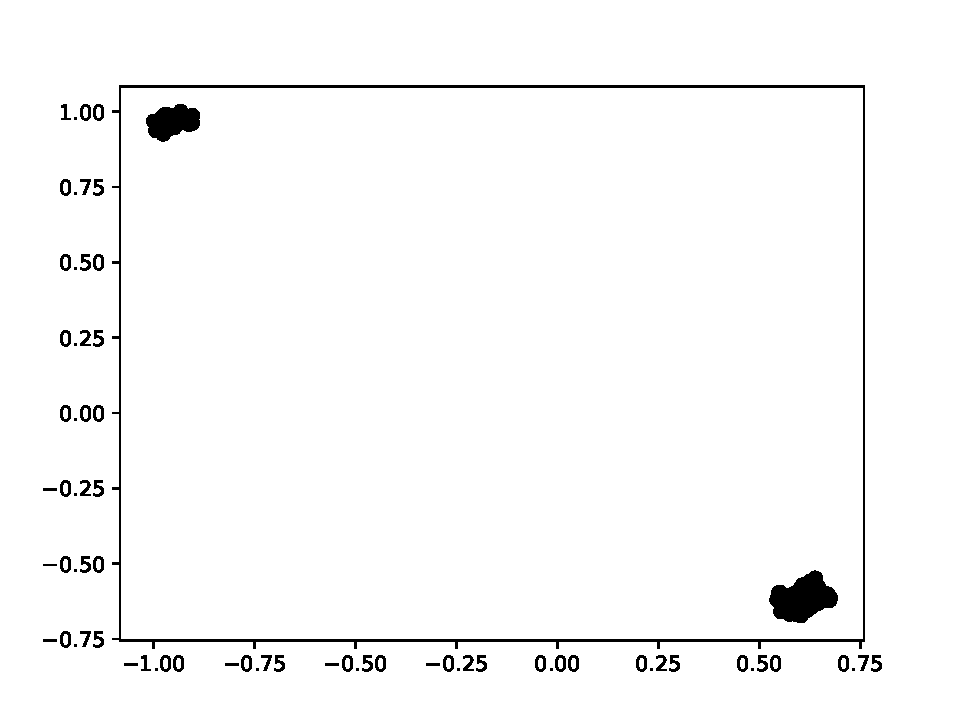
\includegraphics[width=\columnwidth]{figs/embedded-data.pdf}
  \caption{Embedded dataset.}
  \label{fig:emb_dat}
\end{figure}

The results in the following sections were obtained by using the 6-dimensional
dataset. All the procedures were also applied to the embedded 2-dimensional data
(via TSNE) but the results are presented in Appendix \ref{app:emb}.

\subsection{Support Vector Machines}
\begin{figure*}
    \centering
    \begin{subfigure}[b]{0.32\textwidth}
        \centering
        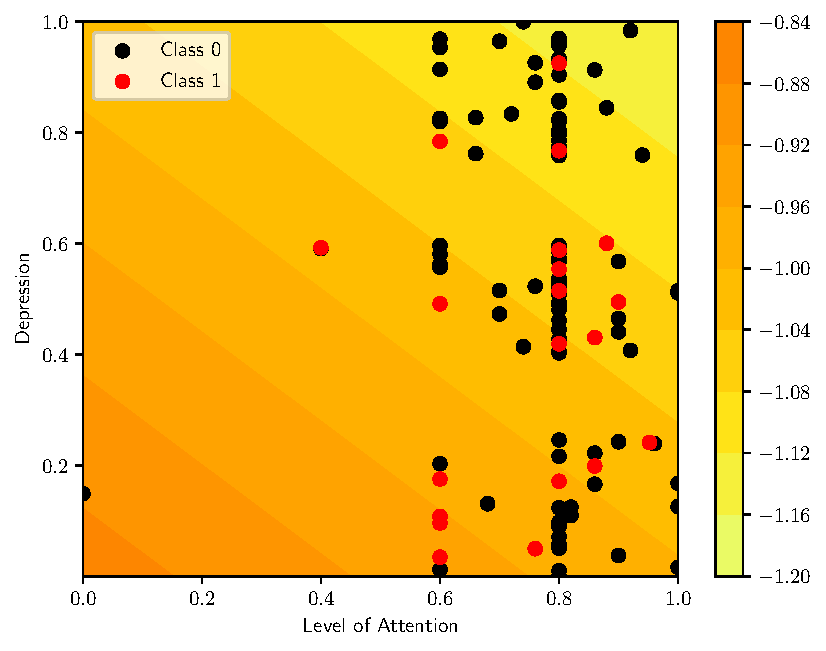
\includegraphics[width=\textwidth]{figs/svm-linear-contour-0-3.pdf}
        \caption{}
    \end{subfigure}
    \begin{subfigure}[b]{0.32\textwidth}
        \centering
        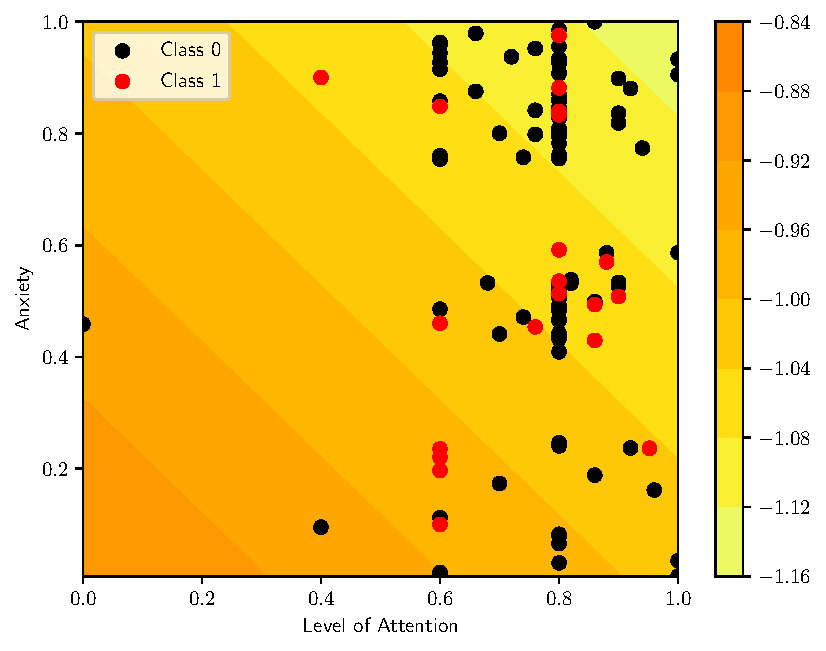
\includegraphics[width=\textwidth]{figs/svm-linear-contour-0-4.pdf}
        \caption{}
    \end{subfigure}
    \begin{subfigure}[b]{0.32\textwidth}
        \centering
        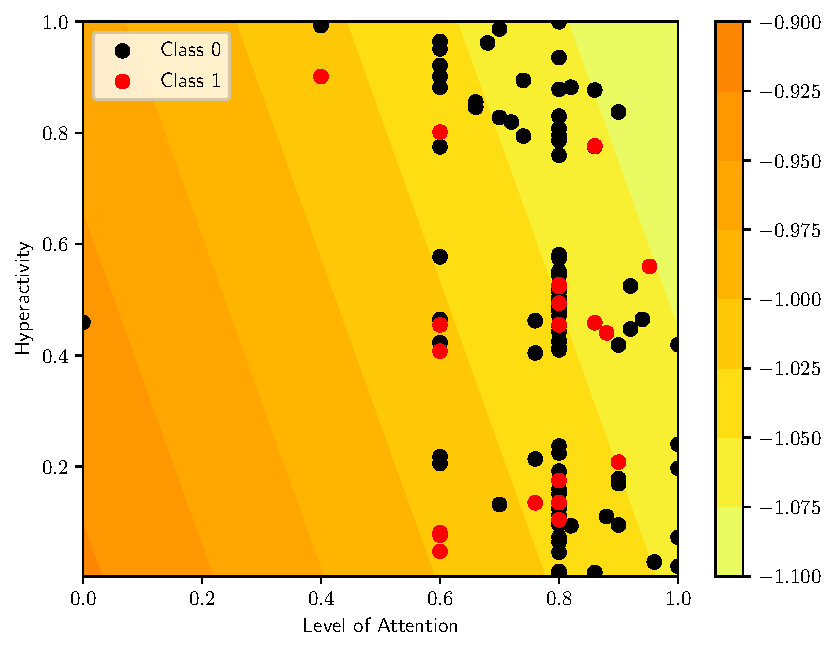
\includegraphics[width=\textwidth]{figs/svm-linear-contour-0-5.pdf}
        \caption{}
    \end{subfigure}

    \begin{subfigure}[b]{0.32\textwidth}
        \centering
        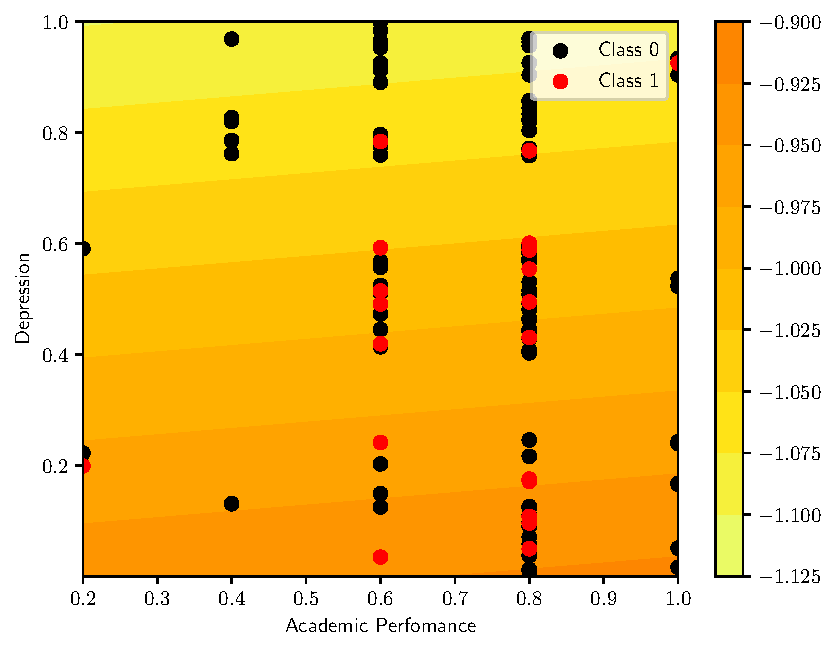
\includegraphics[width=\textwidth]{figs/svm-linear-contour-1-3.pdf}
        \caption{}
    \end{subfigure}
    \begin{subfigure}[b]{0.32\textwidth}
        \centering
        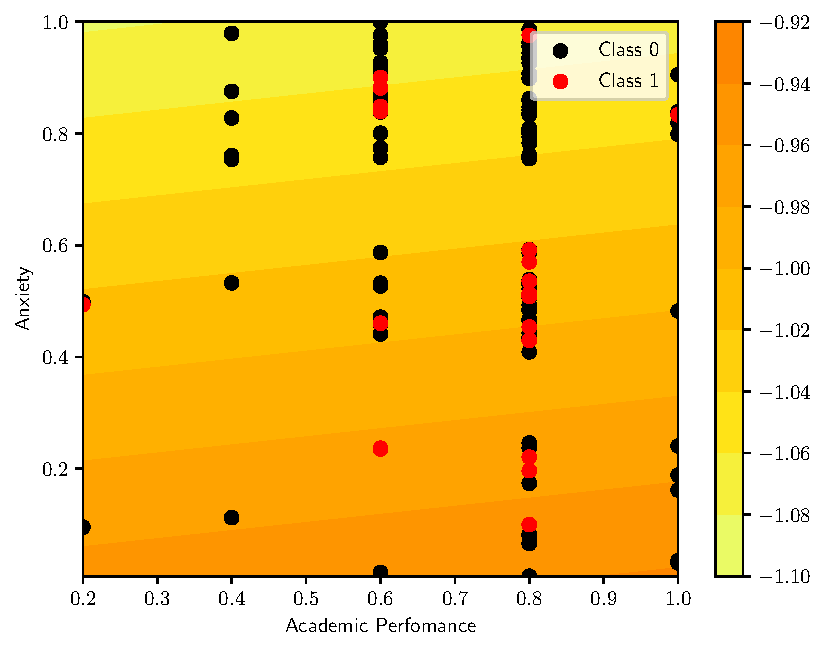
\includegraphics[width=\textwidth]{figs/svm-linear-contour-1-4.pdf}
        \caption{}
    \end{subfigure}
    \begin{subfigure}[b]{0.32\textwidth}
        \centering
        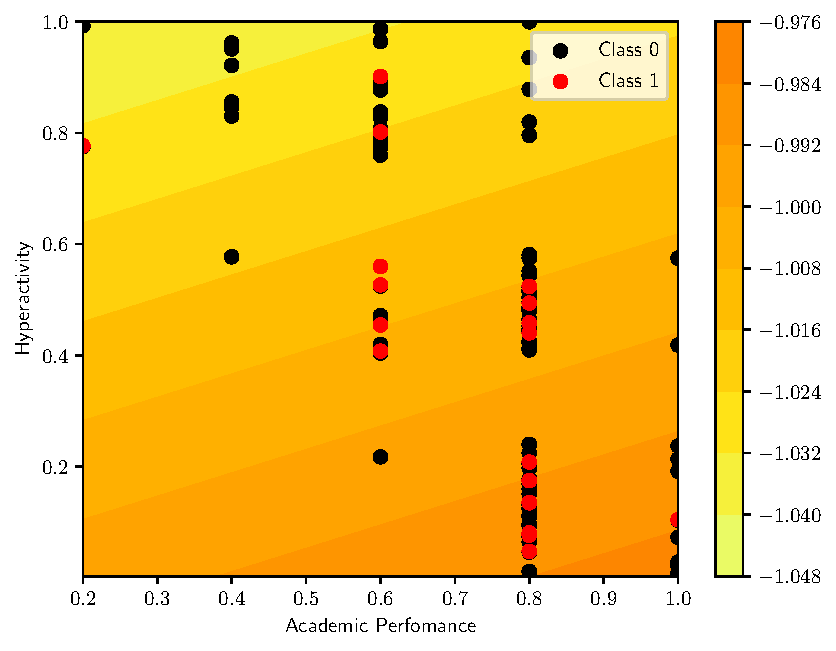
\includegraphics[width=\textwidth]{figs/svm-linear-contour-1-5.pdf}
        \caption{}
    \end{subfigure}

    \begin{subfigure}[b]{0.32\textwidth}
        \centering
        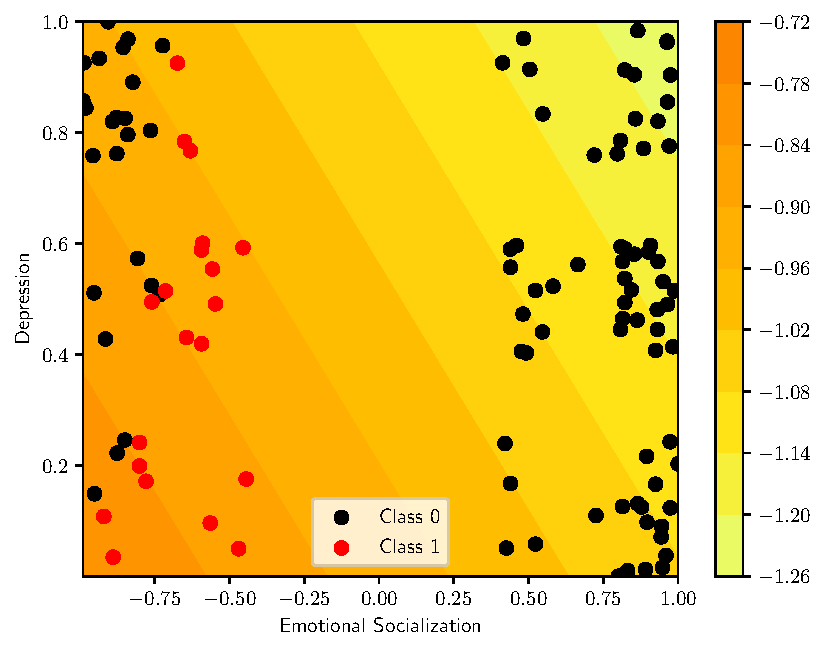
\includegraphics[width=\textwidth]{figs/svm-linear-contour-2-3.pdf}
        \caption{}
    \end{subfigure}
    \begin{subfigure}[b]{0.32\textwidth}
        \centering
        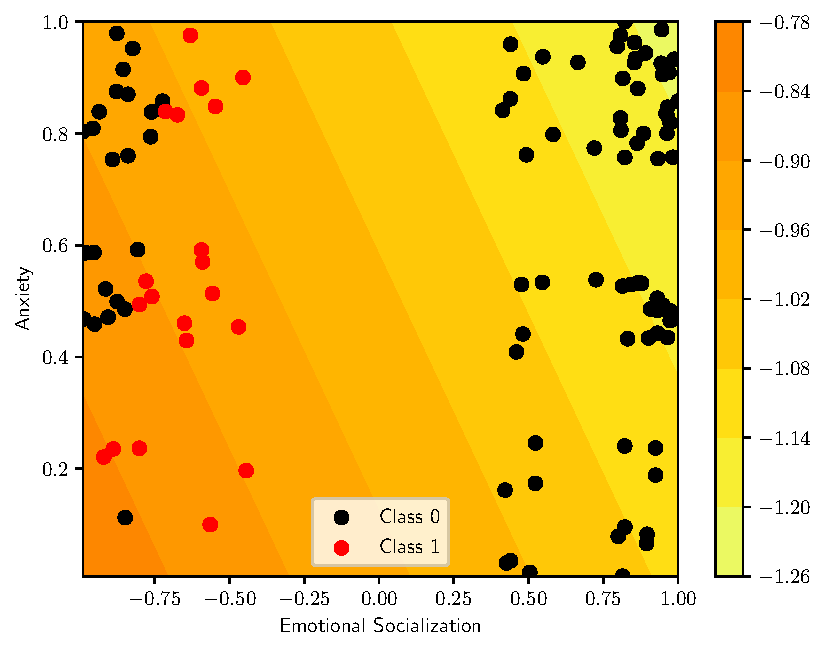
\includegraphics[width=\textwidth]{figs/svm-linear-contour-2-4.pdf}
        \caption{}
    \end{subfigure}
    \begin{subfigure}[b]{0.32\textwidth}
        \centering
        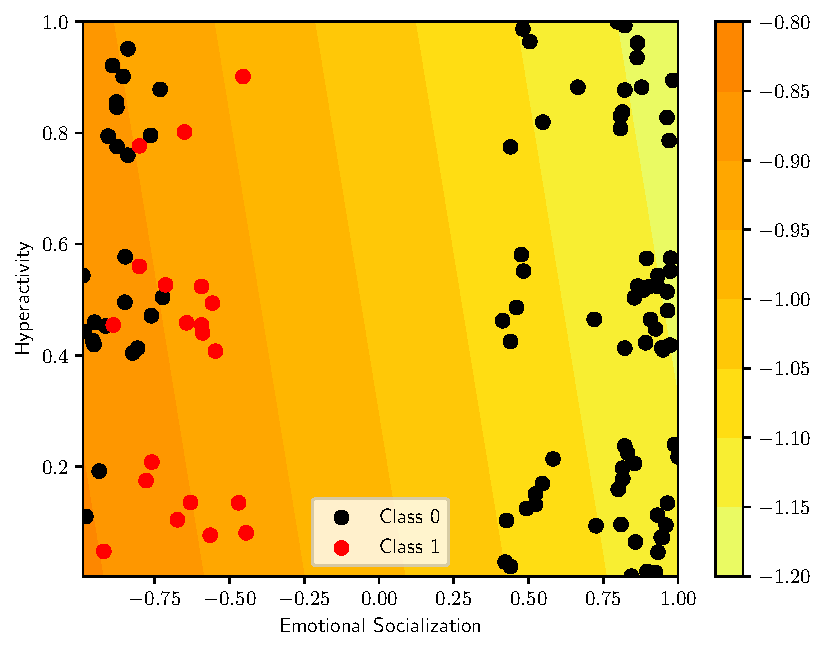
\includegraphics[width=\textwidth]{figs/svm-linear-contour-2-5.pdf}
        \caption{}
    \end{subfigure}
    \caption{Linear kernel SVM contour with real labels.}
    \label{fig:SVM-linear}
\end{figure*}

\begin{figure*}
    \centering
    \begin{subfigure}[b]{0.32\textwidth}
        \centering
        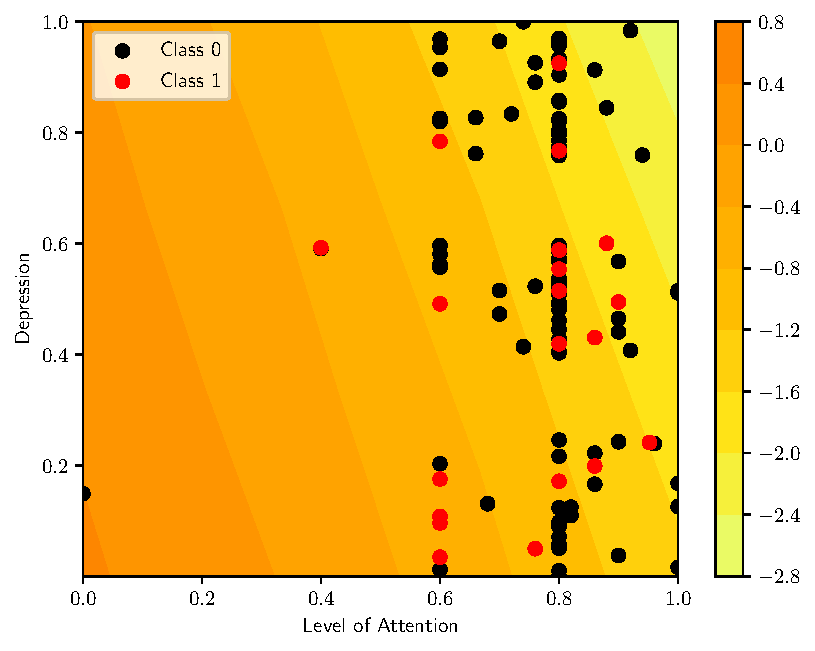
\includegraphics[width=\textwidth]{figs/svm-poly-contour-0-3.pdf}
        \caption{}
    \end{subfigure}
    \begin{subfigure}[b]{0.32\textwidth}
        \centering
        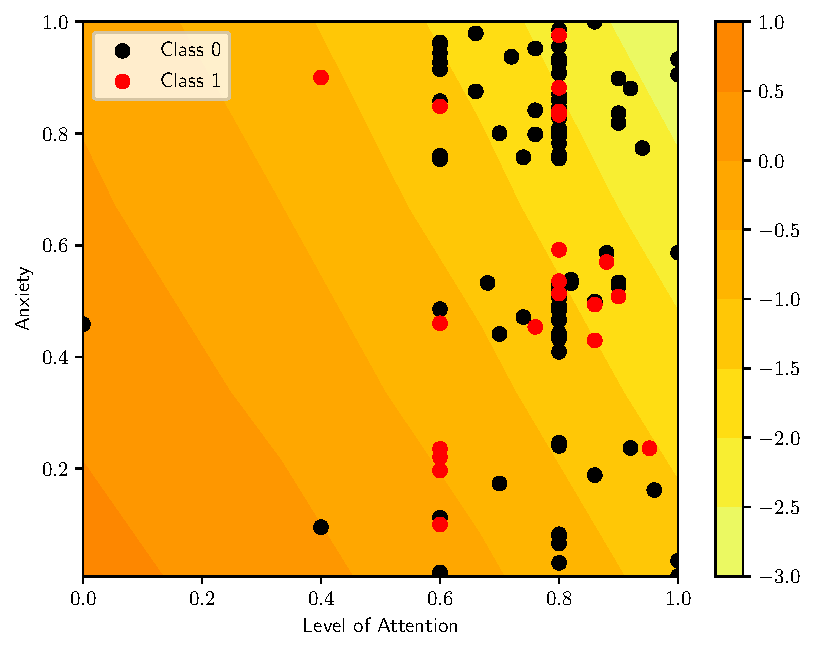
\includegraphics[width=\textwidth]{figs/svm-poly-contour-0-4.pdf}
        \caption{}
    \end{subfigure}
    \begin{subfigure}[b]{0.32\textwidth}
        \centering
        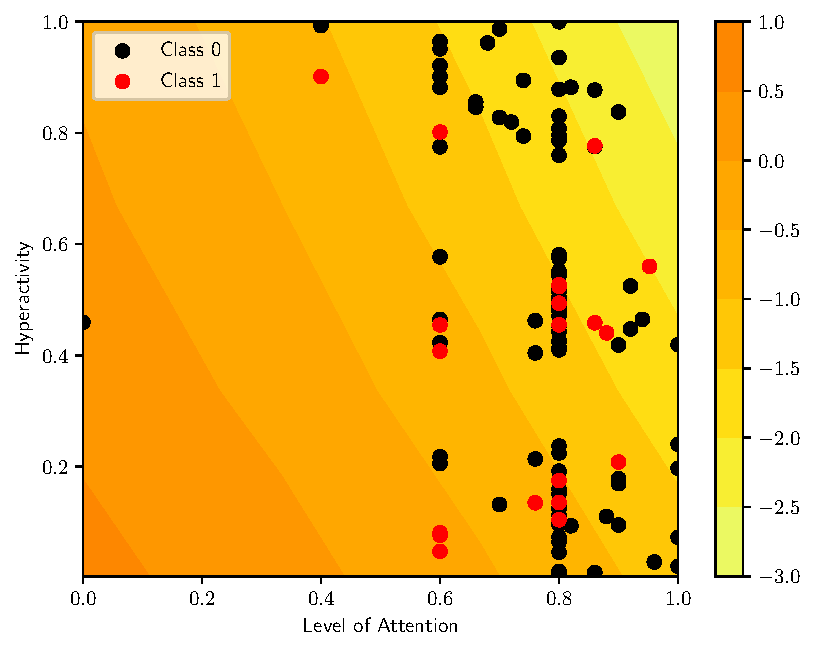
\includegraphics[width=\textwidth]{figs/svm-poly-contour-0-5.pdf}
        \caption{}
    \end{subfigure}

    \begin{subfigure}[b]{0.32\textwidth}
        \centering
        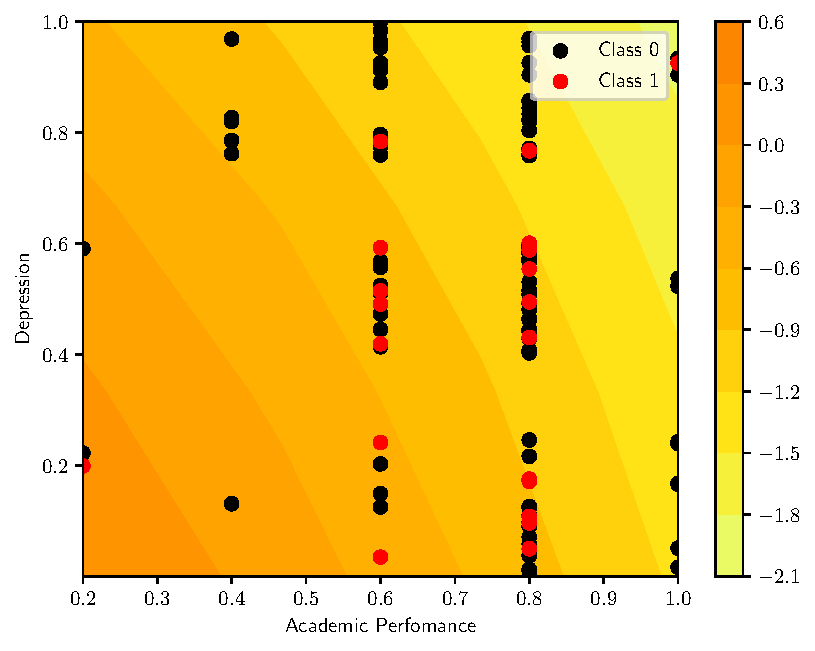
\includegraphics[width=\textwidth]{figs/svm-poly-contour-1-3.pdf}
        \caption{}
    \end{subfigure}
    \begin{subfigure}[b]{0.32\textwidth}
        \centering
        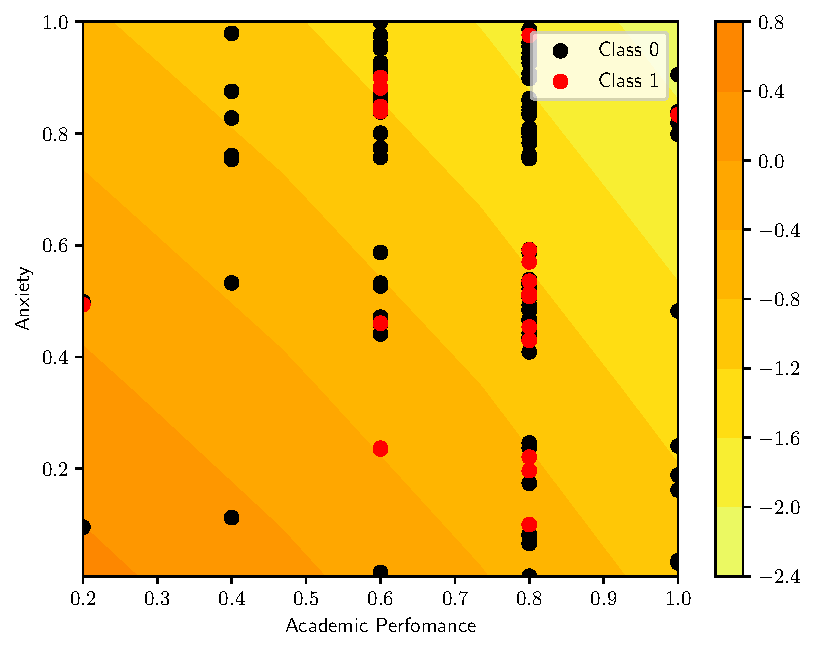
\includegraphics[width=\textwidth]{figs/svm-poly-contour-1-4.pdf}
        \caption{}
    \end{subfigure}
    \begin{subfigure}[b]{0.32\textwidth}
        \centering
        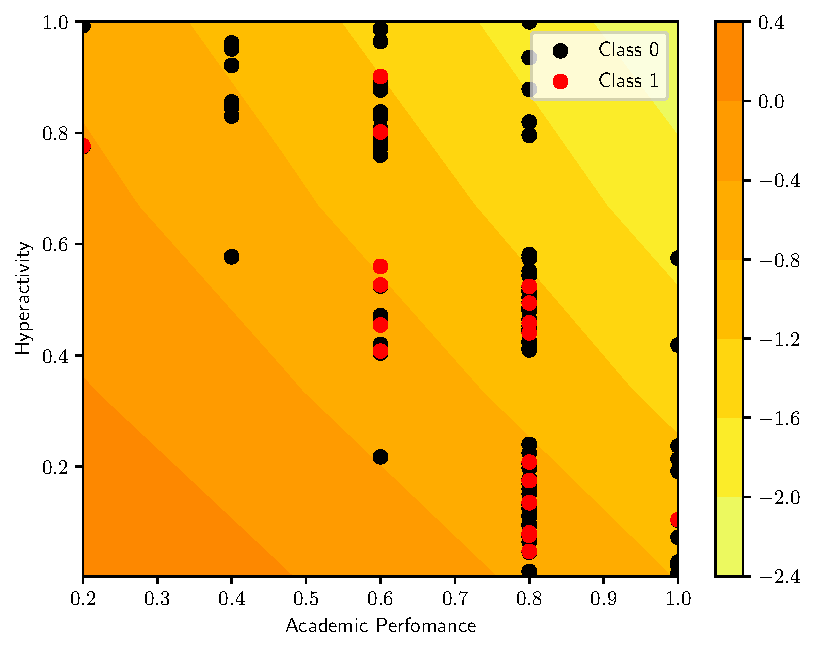
\includegraphics[width=\textwidth]{figs/svm-poly-contour-1-5.pdf}
        \caption{}
    \end{subfigure}

    \begin{subfigure}[b]{0.32\textwidth}
        \centering
        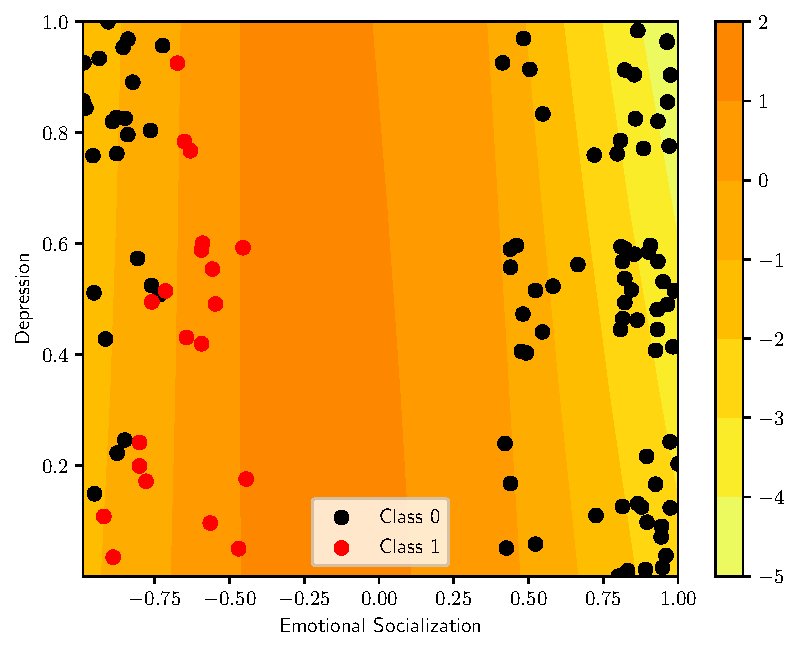
\includegraphics[width=\textwidth]{figs/svm-poly-contour-2-3.pdf}
        \caption{}
    \end{subfigure}
    \begin{subfigure}[b]{0.32\textwidth}
        \centering
        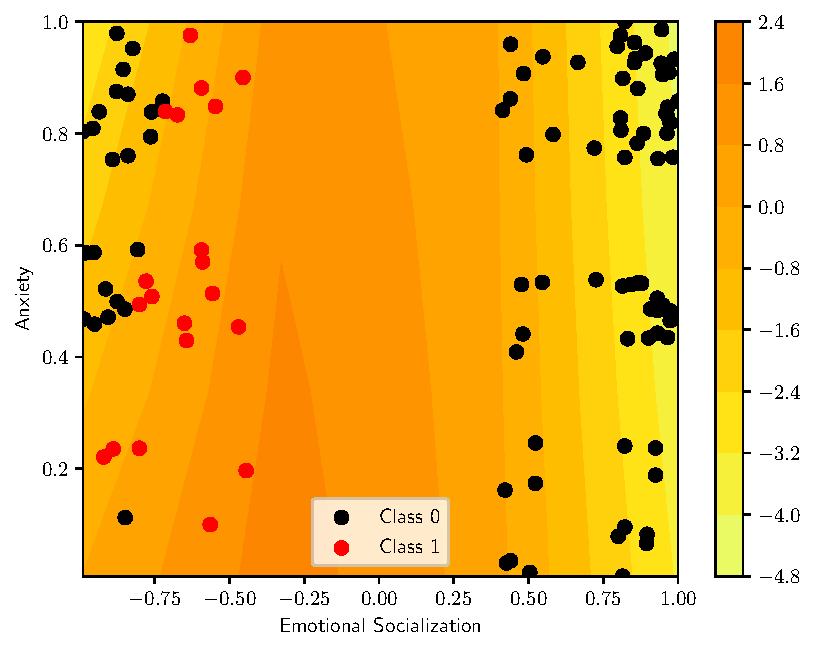
\includegraphics[width=\textwidth]{figs/svm-poly-contour-2-4.pdf}
        \caption{}
    \end{subfigure}
    \begin{subfigure}[b]{0.32\textwidth}
        \centering
        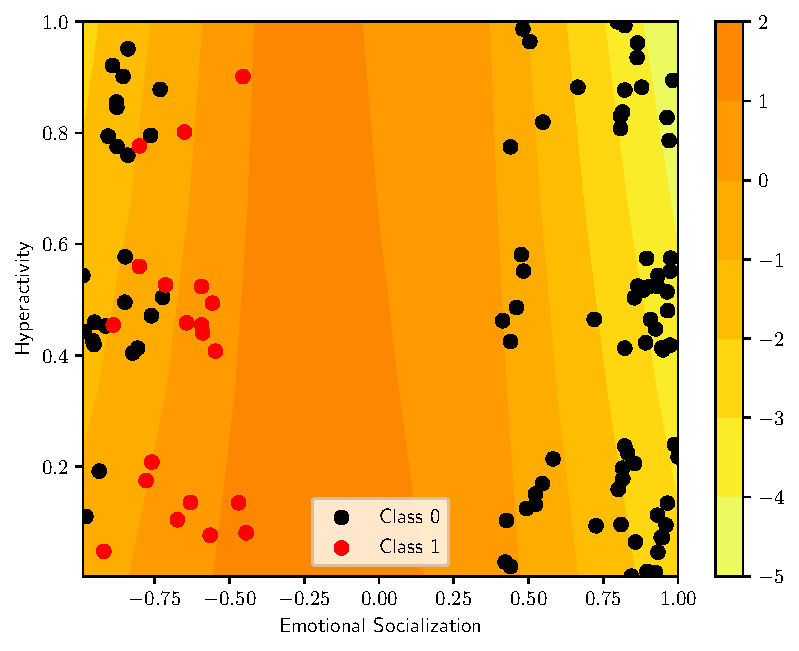
\includegraphics[width=\textwidth]{figs/svm-poly-contour-2-5.pdf}
        \caption{}
    \end{subfigure}
    \caption{Polynomial kernel SVM contour with real labels.}
    \label{fig:SVM-poly}
\end{figure*}

\begin{figure*}
    \centering
    \begin{subfigure}[b]{0.32\textwidth}
        \centering
        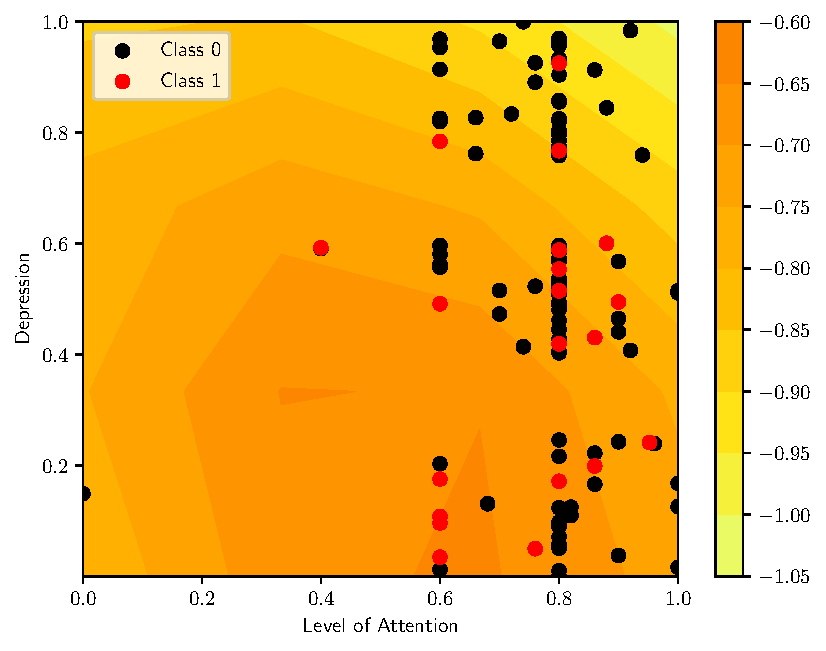
\includegraphics[width=\textwidth]{figs/svm-rbf-contour-0-3.pdf}
        \caption{}
    \end{subfigure}
    \begin{subfigure}[b]{0.32\textwidth}
        \centering
        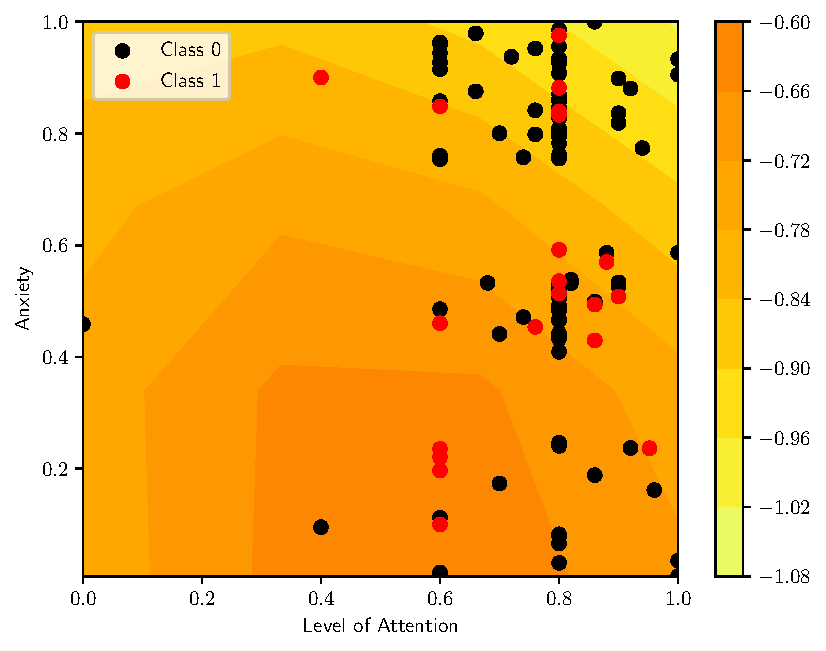
\includegraphics[width=\textwidth]{figs/svm-rbf-contour-0-4.pdf}
        \caption{}
    \end{subfigure}
    \begin{subfigure}[b]{0.32\textwidth}
        \centering
        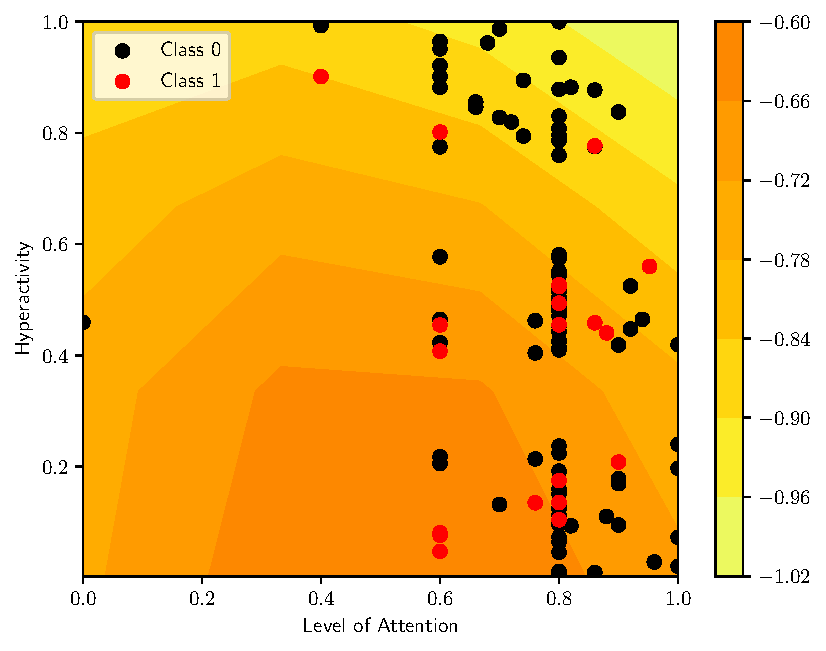
\includegraphics[width=\textwidth]{figs/svm-rbf-contour-0-5.pdf}
        \caption{}
    \end{subfigure}

    \begin{subfigure}[b]{0.32\textwidth}
        \centering
        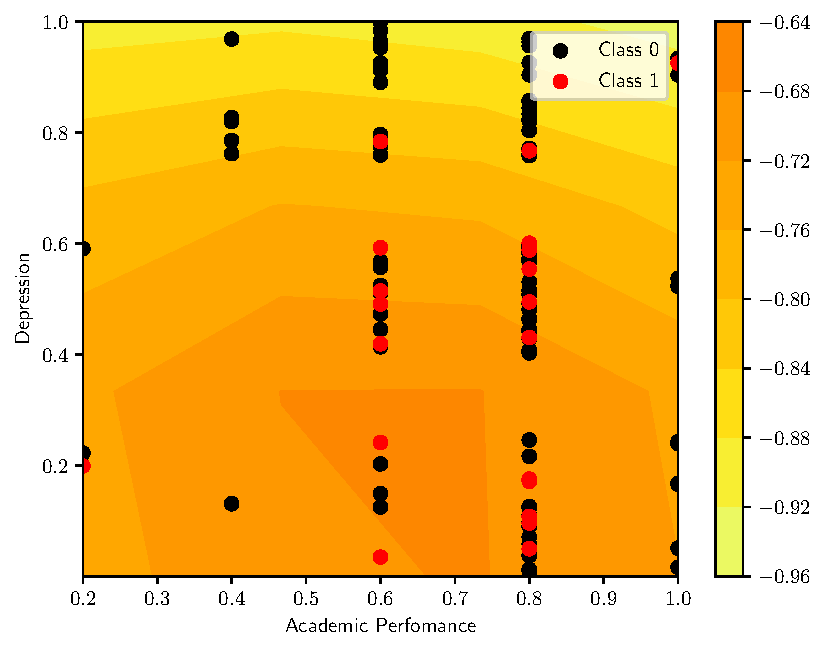
\includegraphics[width=\textwidth]{figs/svm-rbf-contour-1-3.pdf}
        \caption{}
    \end{subfigure}
    \begin{subfigure}[b]{0.32\textwidth}
        \centering
        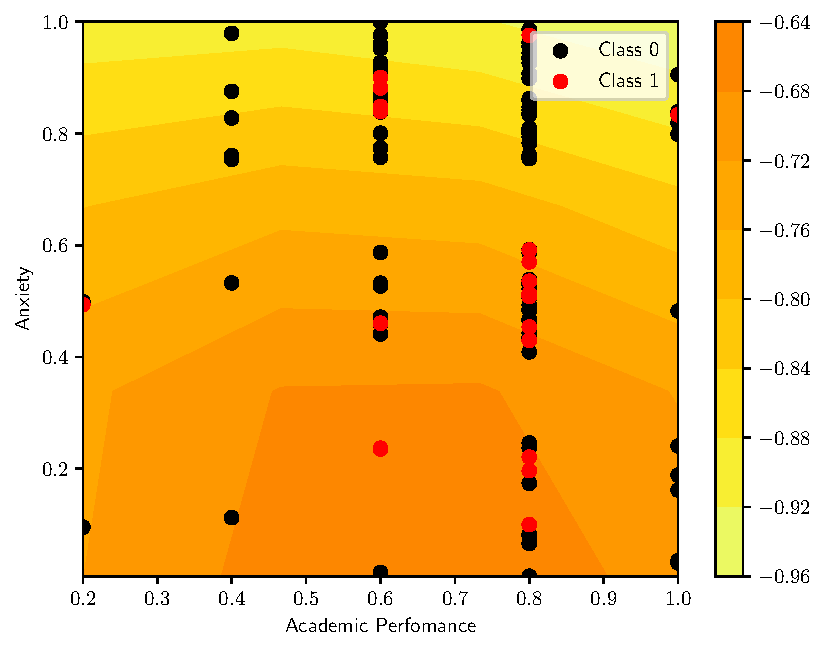
\includegraphics[width=\textwidth]{figs/svm-rbf-contour-1-4.pdf}
        \caption{}
    \end{subfigure}
    \begin{subfigure}[b]{0.32\textwidth}
        \centering
        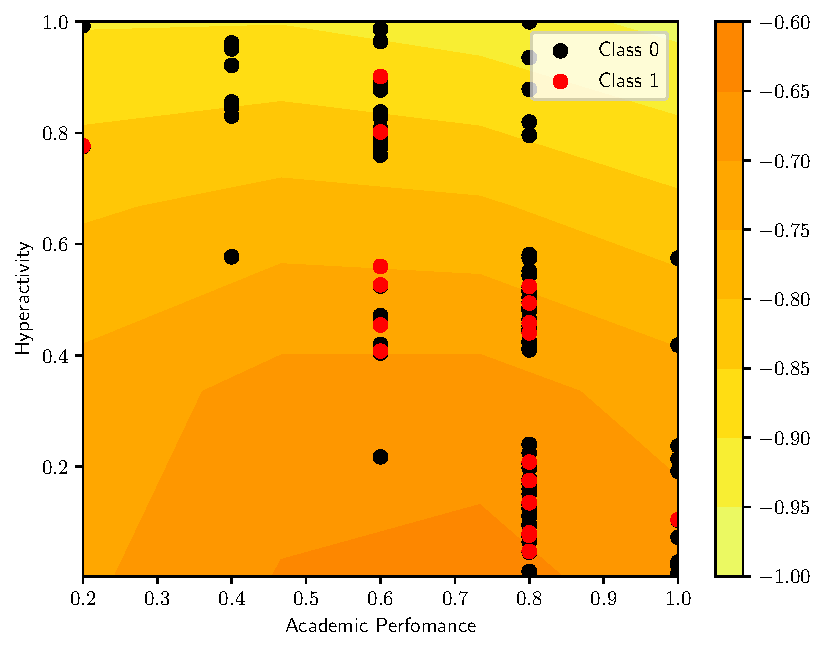
\includegraphics[width=\textwidth]{figs/svm-rbf-contour-1-5.pdf}
        \caption{}
    \end{subfigure}

    \begin{subfigure}[b]{0.32\textwidth}
        \centering
        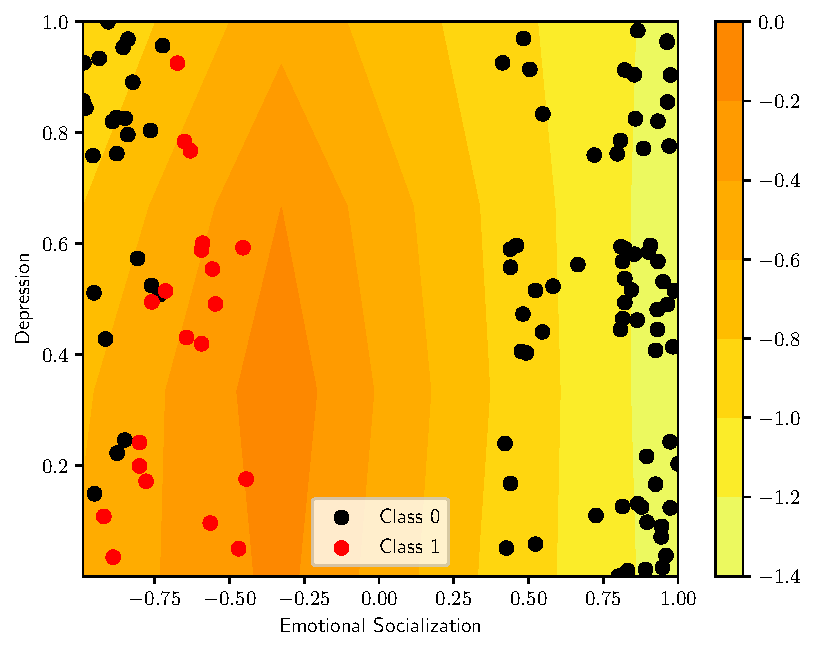
\includegraphics[width=\textwidth]{figs/svm-rbf-contour-2-3.pdf}
        \caption{}
    \end{subfigure}
    \begin{subfigure}[b]{0.32\textwidth}
        \centering
        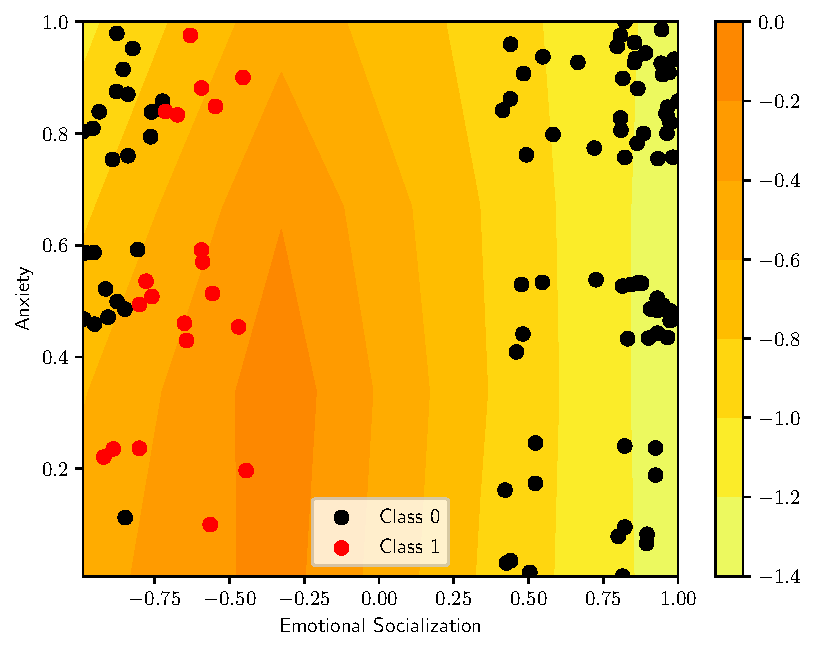
\includegraphics[width=\textwidth]{figs/svm-rbf-contour-2-4.pdf}
        \caption{}
    \end{subfigure}
    \begin{subfigure}[b]{0.32\textwidth}
        \centering
        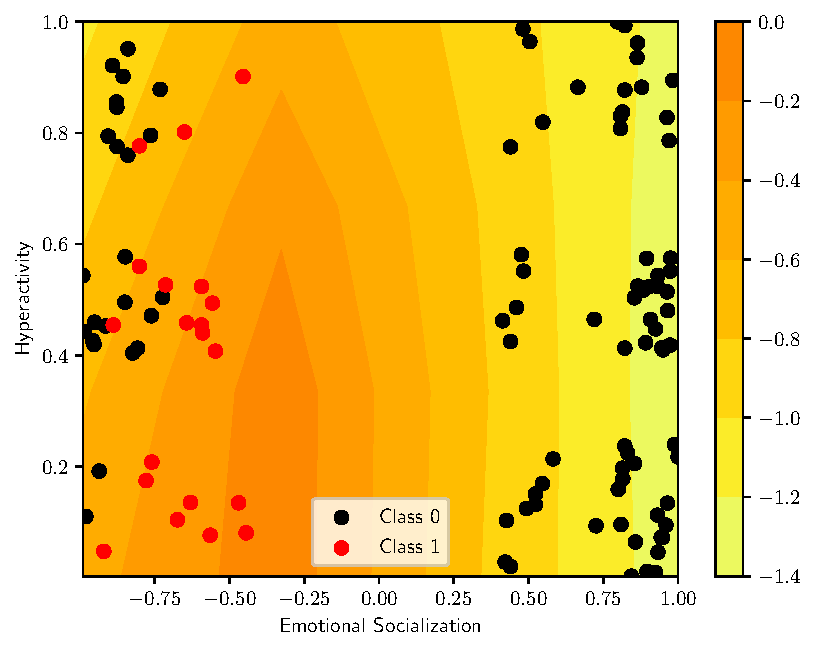
\includegraphics[width=\textwidth]{figs/svm-rbf-contour-2-5.pdf}
        \caption{}
    \end{subfigure}
    \caption{RBF kernel SVM contour with real labels.}
    \label{fig:SVM-rbf}
\end{figure*}

\begin{table}
\centering
\caption{Performance scores for linear SVM.}
\label{tab:linear_SVM}
\begin{tabular}{ccc}
\hline
\textbf{Set} & \textbf{Sensitivity} & \textbf{Specificity} \\ \hline
Training & 0 & 1 \\
Testing & 0 & 1 \\
Validation & 0 & 1 \\ \hline
\end{tabular}
\end{table}

\begin{table}
\centering
\caption{Performance scores for polynomial SVM.}
\label{tab:poly_SVM}
\begin{tabular}{cll}
\hline
\textbf{Set} & \multicolumn{1}{c}{\textbf{Sensitivity}} & \multicolumn{1}{c}{\textbf{Specificity}} \\ \hline
Training & 0.89 & 1 \\
Testing & 0 & 1 \\
Validation & 0.57 & 1 \\ \hline
\end{tabular}
\end{table}

\begin{table}
\centering
\caption{Performance scores for RBF SVM.}
\label{tab:rbf_SVM}
\begin{tabular}{cll}
\hline
\textbf{Set} & \multicolumn{1}{c}{\textbf{Sensitivity}} & \multicolumn{1}{c}{\textbf{Specificity}} \\ \hline
Training & 0.13 & 1 \\
Testing & 0 & 1 \\
Validation & 0.25 & 1 \\ \hline
\end{tabular}
\end{table}


\subsection{Decision Trees}
\begin{figure}
    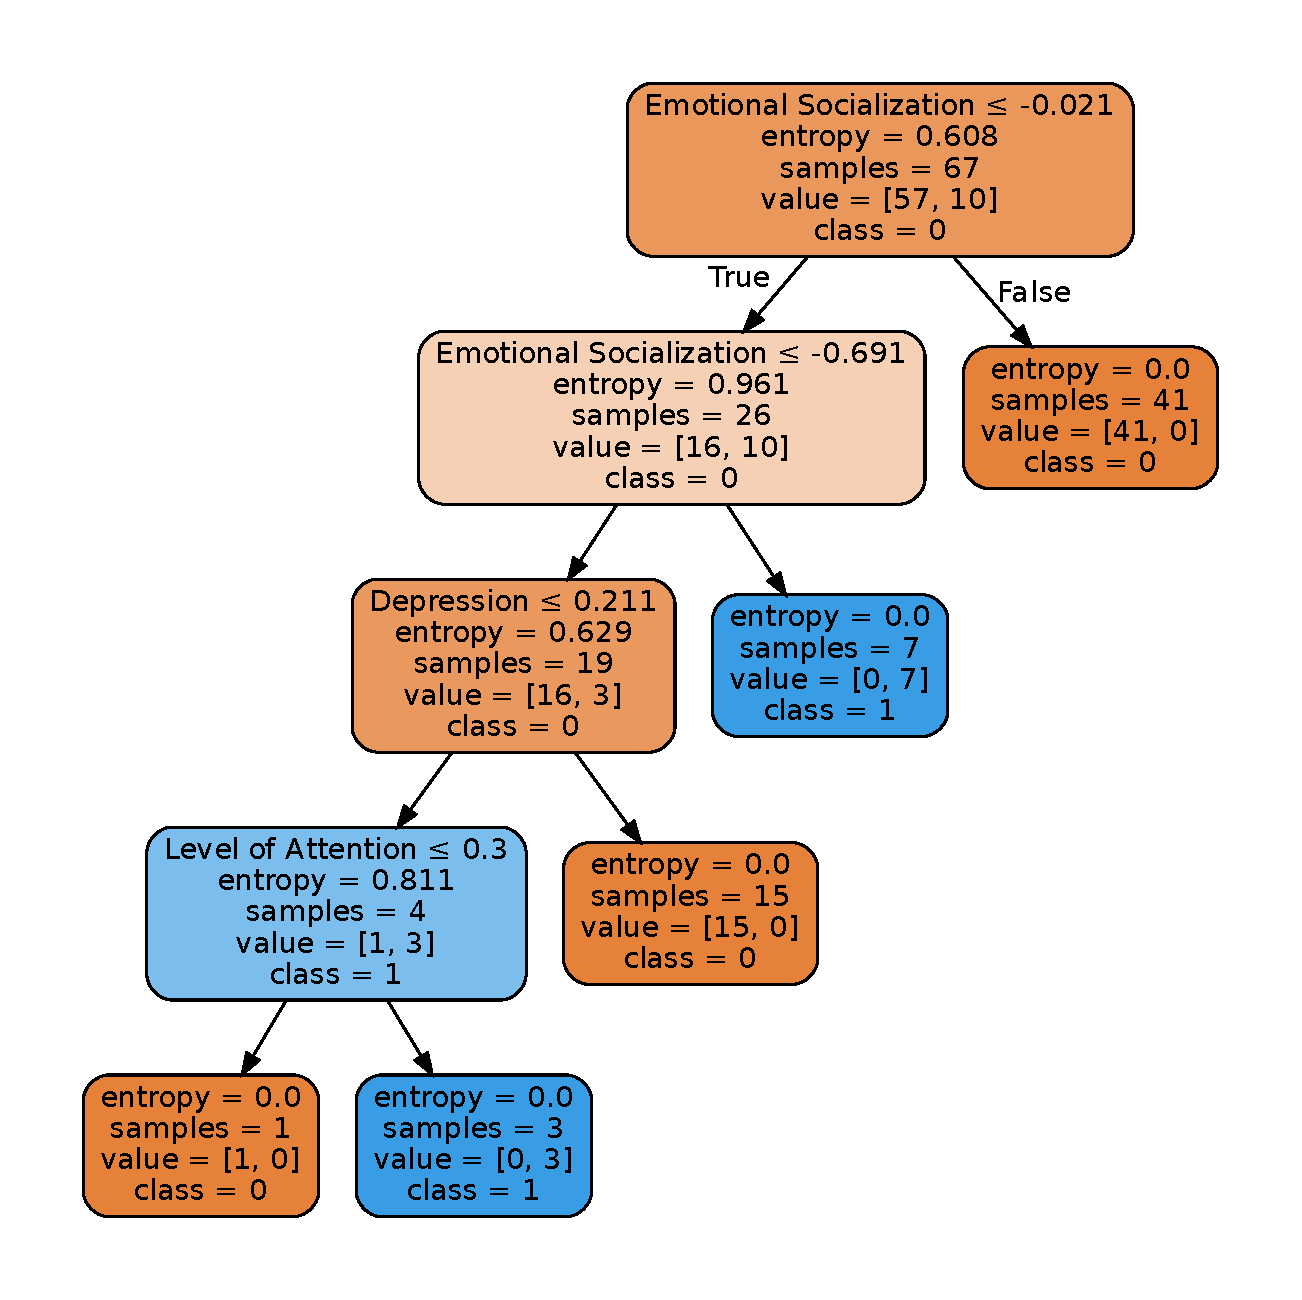
\includegraphics[width=\columnwidth]{figs/tree-graph.pdf}
    \caption{Decision tree.}
    \label{fig:dt}
\end{figure}

\begin{figure*}
    \centering
    \begin{subfigure}[b]{0.32\textwidth}
        \centering
        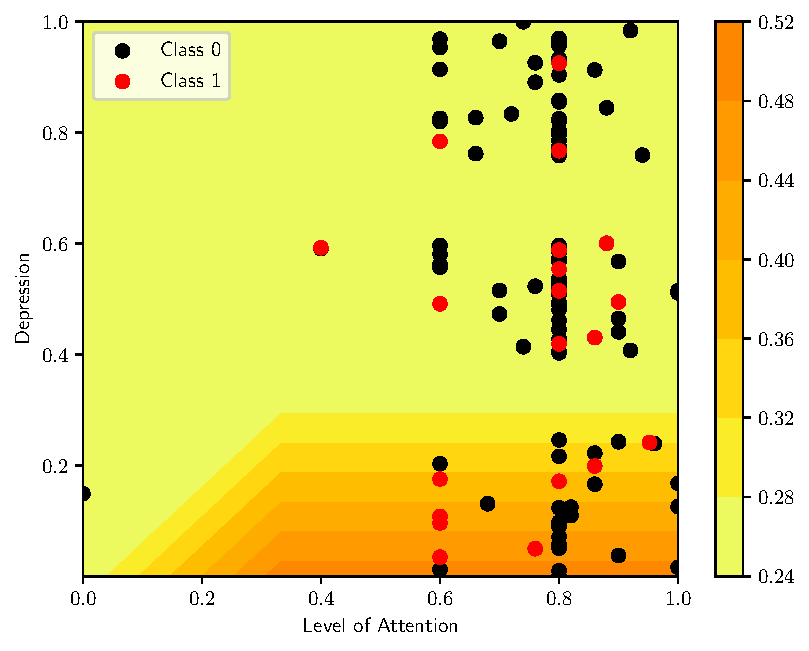
\includegraphics[width=\textwidth]{figs/tree-contour-0-3.pdf}
        \caption{}
    \end{subfigure}
    \begin{subfigure}[b]{0.32\textwidth}
        \centering
        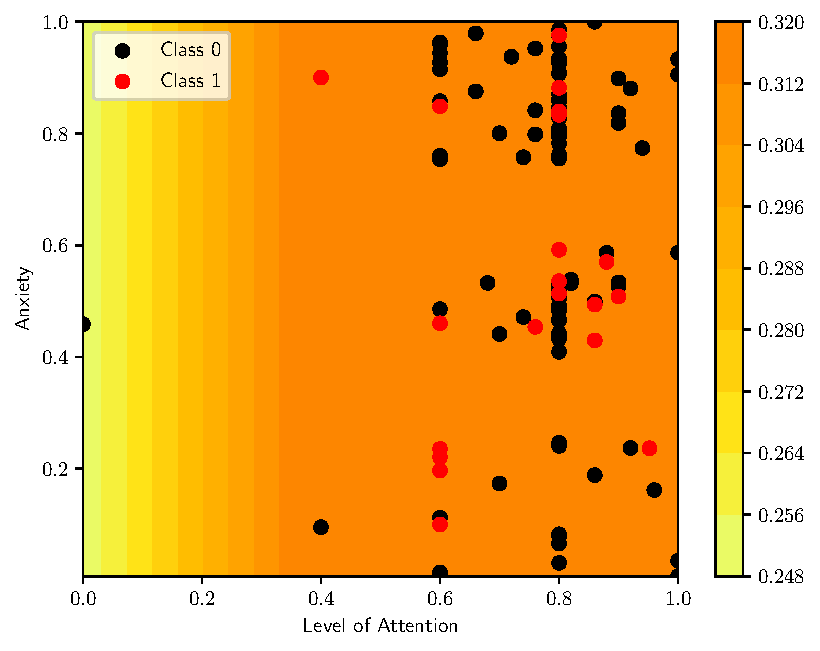
\includegraphics[width=\textwidth]{figs/tree-contour-0-4.pdf}
        \caption{}
    \end{subfigure}
    \begin{subfigure}[b]{0.32\textwidth}
        \centering
        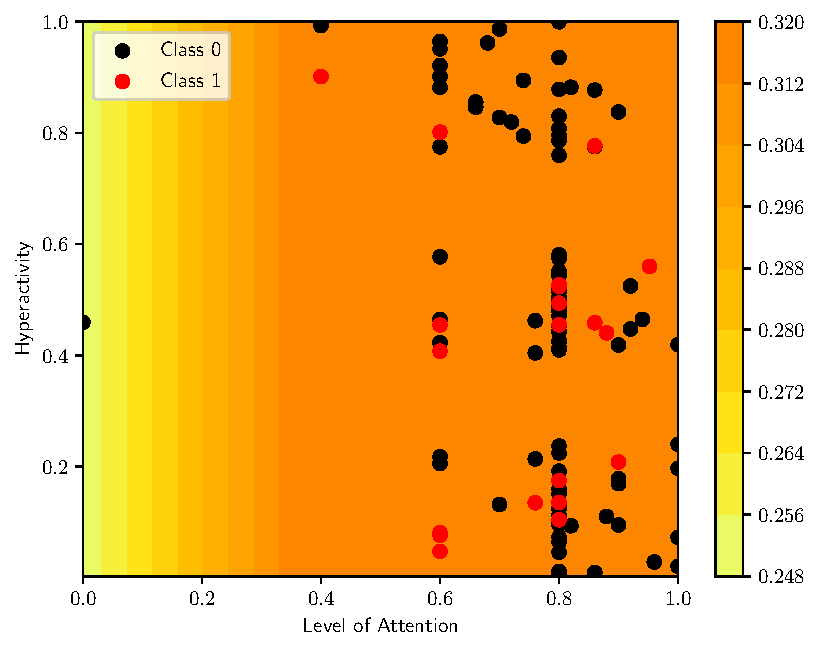
\includegraphics[width=\textwidth]{figs/tree-contour-0-5.pdf}
        \caption{}
    \end{subfigure}

    \begin{subfigure}[b]{0.32\textwidth}
        \centering
        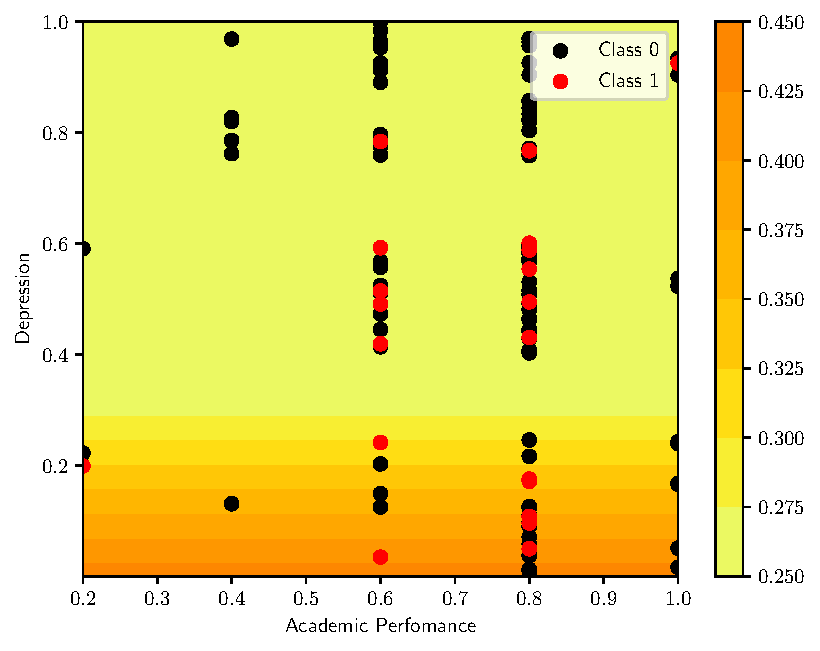
\includegraphics[width=\textwidth]{figs/tree-contour-1-3.pdf}
        \caption{}
    \end{subfigure}
    \begin{subfigure}[b]{0.32\textwidth}
        \centering
        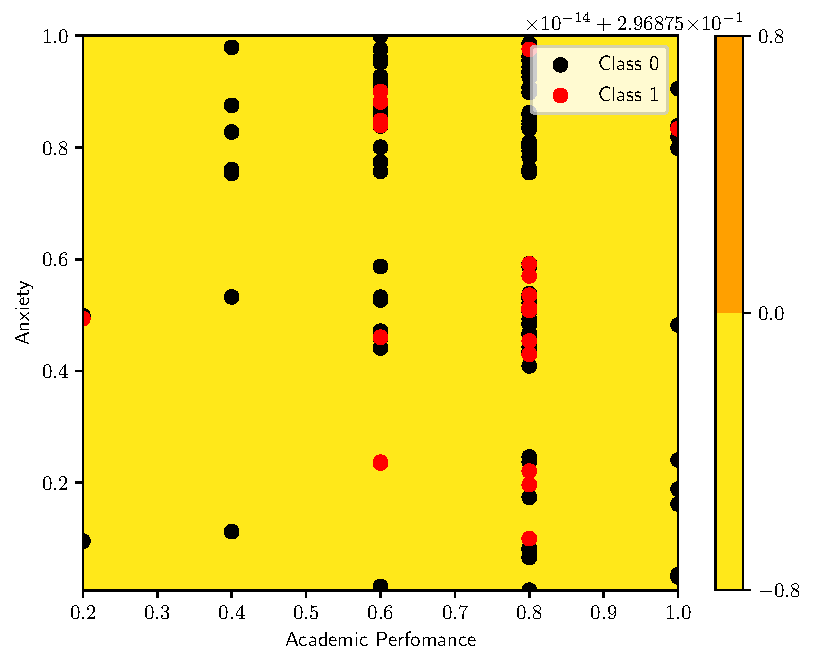
\includegraphics[width=\textwidth]{figs/tree-contour-1-4.pdf}
        \caption{}
    \end{subfigure}
    \begin{subfigure}[b]{0.32\textwidth}
        \centering
        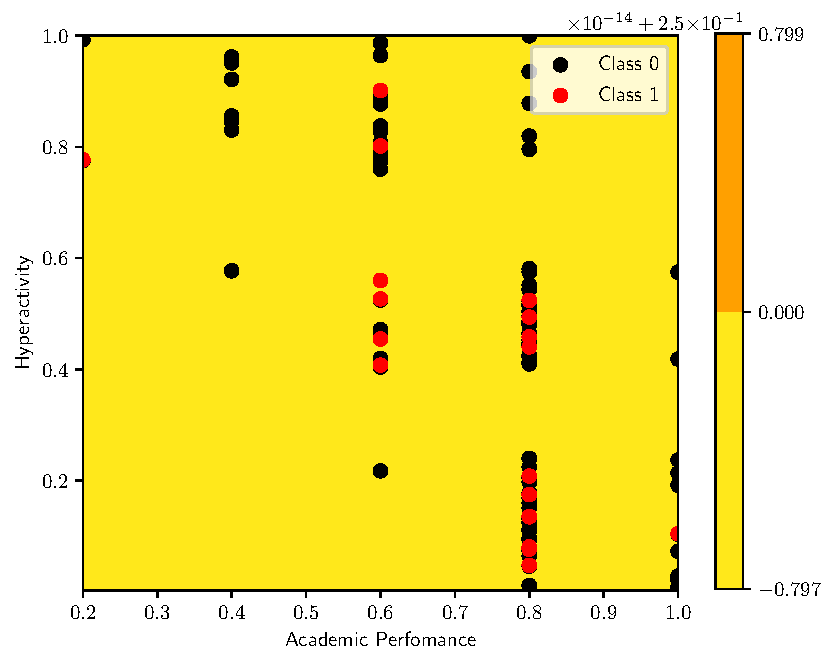
\includegraphics[width=\textwidth]{figs/tree-contour-1-5.pdf}
        \caption{}
    \end{subfigure}

    \begin{subfigure}[b]{0.32\textwidth}
        \centering
        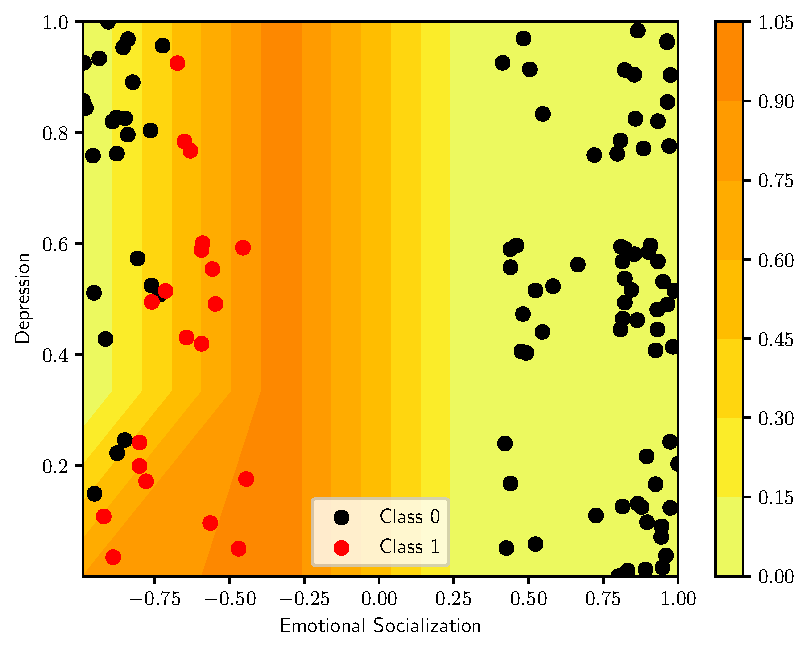
\includegraphics[width=\textwidth]{figs/tree-contour-2-3.pdf}
        \caption{}
    \end{subfigure}
    \begin{subfigure}[b]{0.32\textwidth}
        \centering
        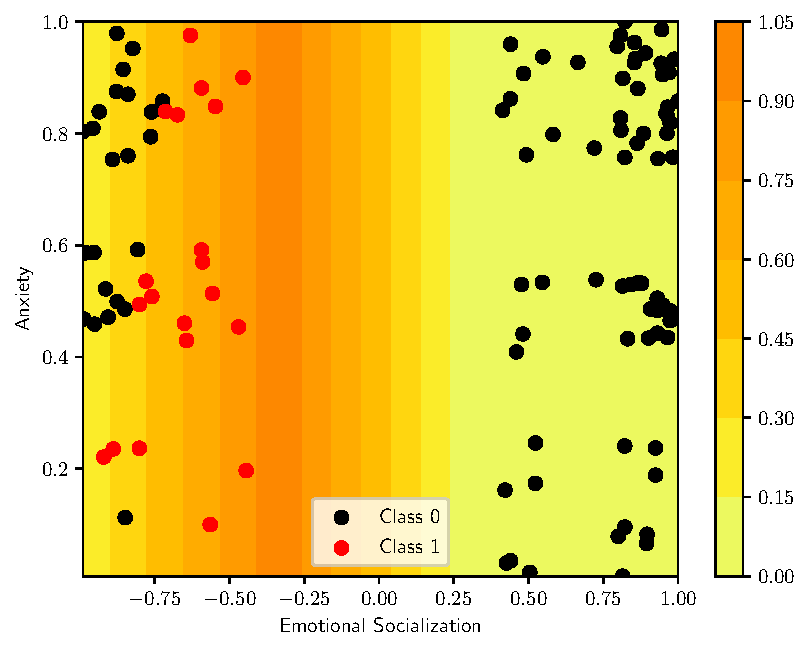
\includegraphics[width=\textwidth]{figs/tree-contour-2-4.pdf}
        \caption{}
    \end{subfigure}
    \begin{subfigure}[b]{0.32\textwidth}
        \centering
        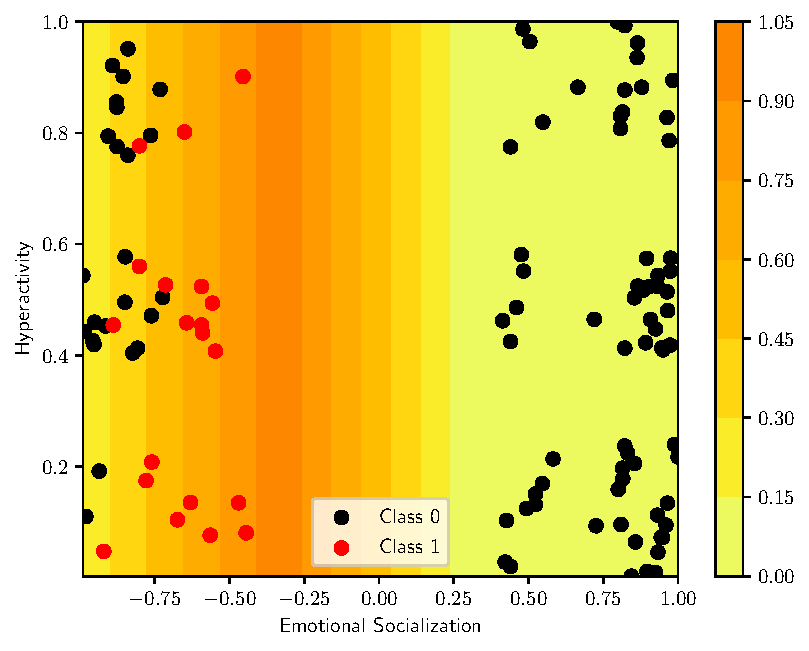
\includegraphics[width=\textwidth]{figs/tree-contour-2-5.pdf}
        \caption{}
    \end{subfigure}
    \caption{Decision Tree contour with real labels.}
    \label{fig:dts}
\end{figure*}

\begin{table}
\centering
\caption{Performance scores for DT.}
\label{tab:DT}
\begin{tabular}{ccc}
\hline
\textbf{Set} & \multicolumn{1}{c}{\textbf{Sensitivity}} & \multicolumn{1}{c}{\textbf{Specificity}} \\ \hline
Training & 1 & 1 \\
Testing & 0.5 & 1 \\
Validation & 0.75 & 1 \\ \hline
\end{tabular}
\end{table}


\subsection{Neural Networks}
Recall that only the worst and 2 best NN are kept for presenting the results.
The worst NN (in the sense of the objective function) was trained with
$\eta=0.9$ and it has a $\mathcal{L}=[1,2,3]$ architecture in the hidden layers.
The learning curves for this MLP are presented in Fig. \ref{fig:NN-worst}. This
architecture is expected to perform poorly, at least for the given number of
epochs, since it is attempting to summarize all 6 inputs in a one dimensional
value for the first hidden layer and then casting this value into higher
dimensions. It is unknown for the authors if this machine can learn the data at
all, since the behavior of the backpropagation algorithm is unpredictable as
epochs advance. Note from Fig. \ref{subfig:grad-worst-NN}, the gradients are
stable in the epoch horizon defined, from Fig. \ref{subfig:error-worst-NN} that
the average energy error seems to reach a stable point, but different from 0,
finally, from Fig. \ref{subfig:roc-worst-NN}, the ROC curve and AUC confirms the
poor performance of this classifier. Finally, the Sensitivity-Specificity
results (see Table \ref{tab:L123}) show that this NN has adequate values for the
specificity but deplorable values for the sensitivity.

\begin{figure*}
  \centering
  \begin{subfigure}[b]{0.32\textwidth}
    \centering 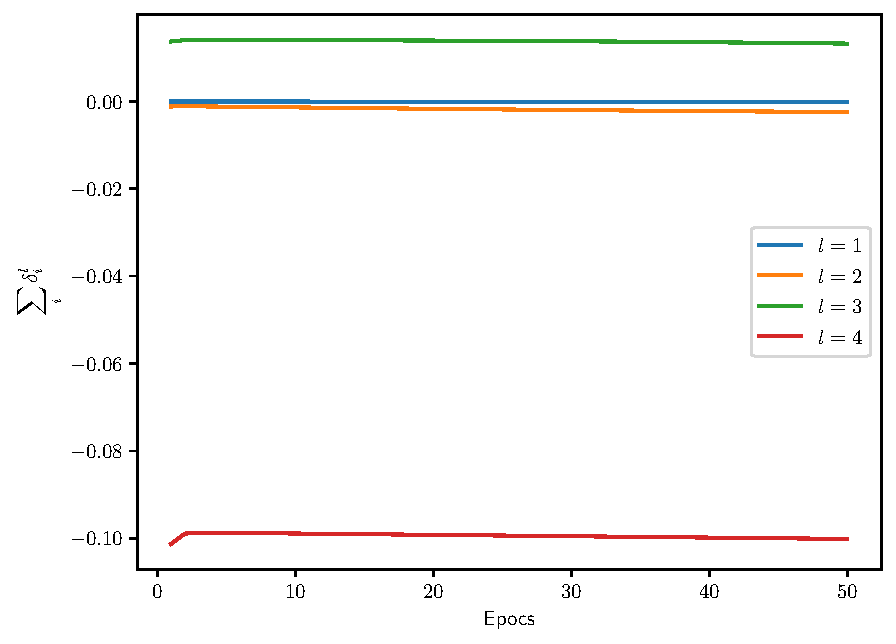
\includegraphics[width=\textwidth]{figs/1-2-3-0.9-gradients.pdf}
    \caption{Gradients for each layer.}
    \label{subfig:grad-worst-NN}
  \end{subfigure}
  \begin{subfigure}[b]{0.32\textwidth}
    \centering 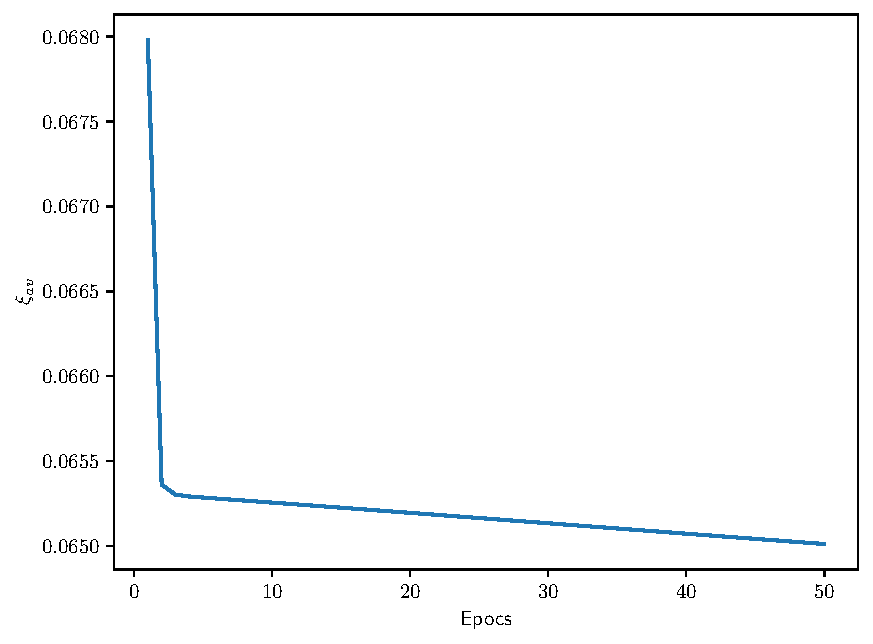
\includegraphics[width=\textwidth]{figs/1-2-3-0.9-error.pdf}
    \caption{Average error energy per epoch.}
    \label{subfig:error-worst-NN}
  \end{subfigure}
  \begin{subfigure}[b]{0.32\textwidth}
    \centering 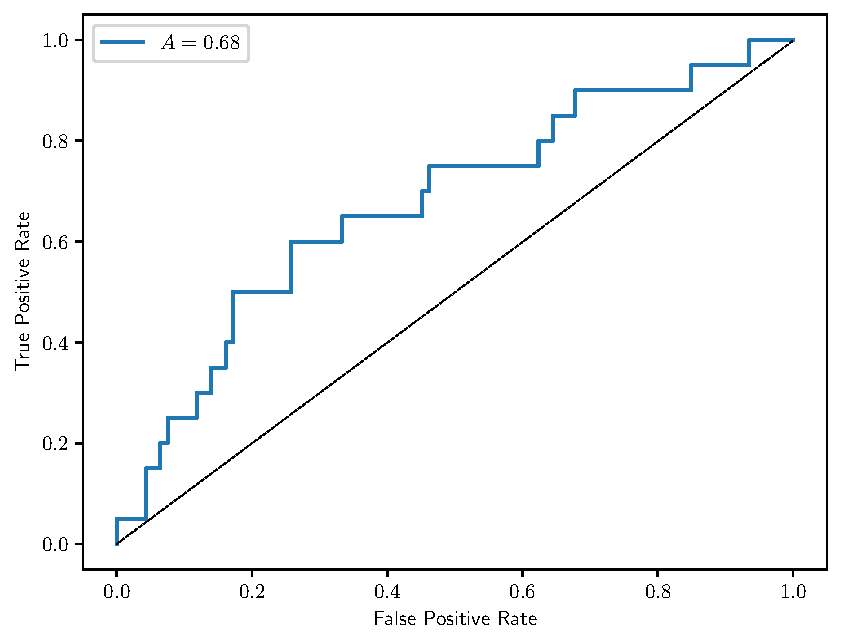
\includegraphics[width=\textwidth]{figs/1-2-3-0.9-roc.pdf}
    \caption{ROC curve.}
    \label{subfig:roc-worst-NN}
  \end{subfigure}
  \caption{Learning curves for $\mathcal{L}=[1,2,3]$ network $\eta=0.9$
    (worst).}
  \label{fig:NN-worst}
\end{figure*}

Furthermore, the second-best NN was obtained with $\mathcal{L}=[2]$ and the best
with $\mathcal{L}=[3]$, both trained with $\eta=0.9$. It is believed that this
MLP obtained better results since the number of weights to optimize was
relatively low and, hence, the backpropagation algorithm converges quickly
(taking into consideration) the elevated learning rate. The training curves for
these two models are presented respectively in Figs. \ref{fig:NN-2best} and
\ref{fig:NN-best}. Note that both networks show rich dynamics on the gradients
through the training stage, the average error energy seems to be descending into
0 and both ROC curves are close to the perfect constant value of 1. The
Sensitivity-Specificity values also show good results on all three sets for the
$\mathcal{L}=3$ architecture.

\begin{figure*}
  \centering
  \begin{subfigure}[b]{0.32\textwidth}
    \centering 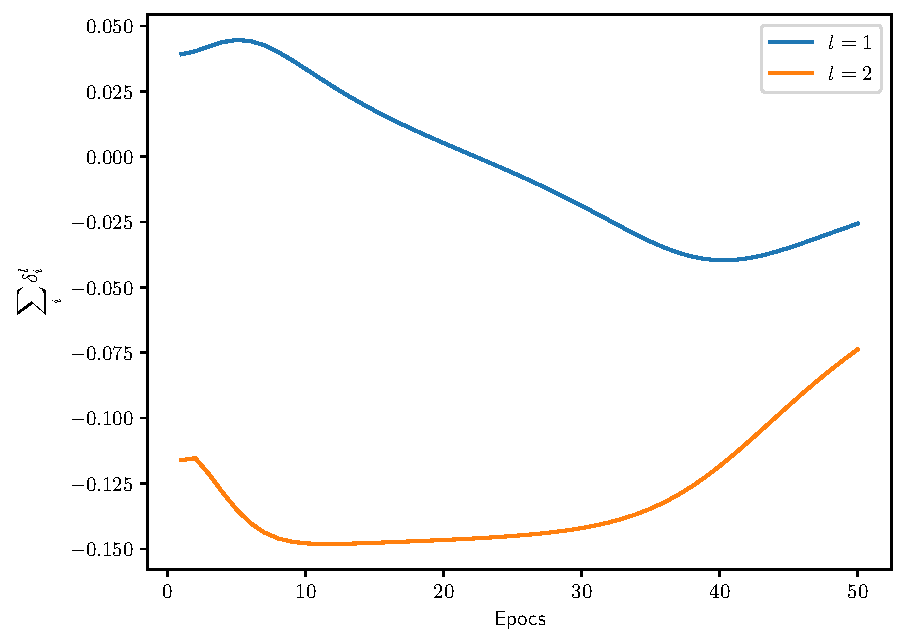
\includegraphics[width=\textwidth]{figs/2-0.9-gradients.pdf}
    \caption{Gradients for each layer.}
  \end{subfigure}
  \begin{subfigure}[b]{0.32\textwidth}
    \centering 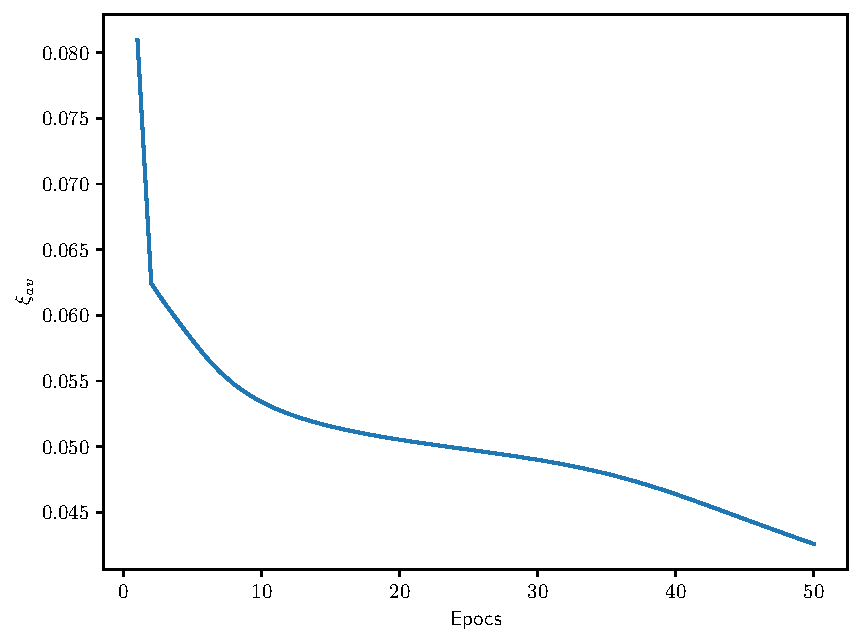
\includegraphics[width=\textwidth]{figs/2-0.9-error.pdf}
    \caption{Average error energy per epoch.}
  \end{subfigure}
  \begin{subfigure}[b]{0.32\textwidth}
    \centering 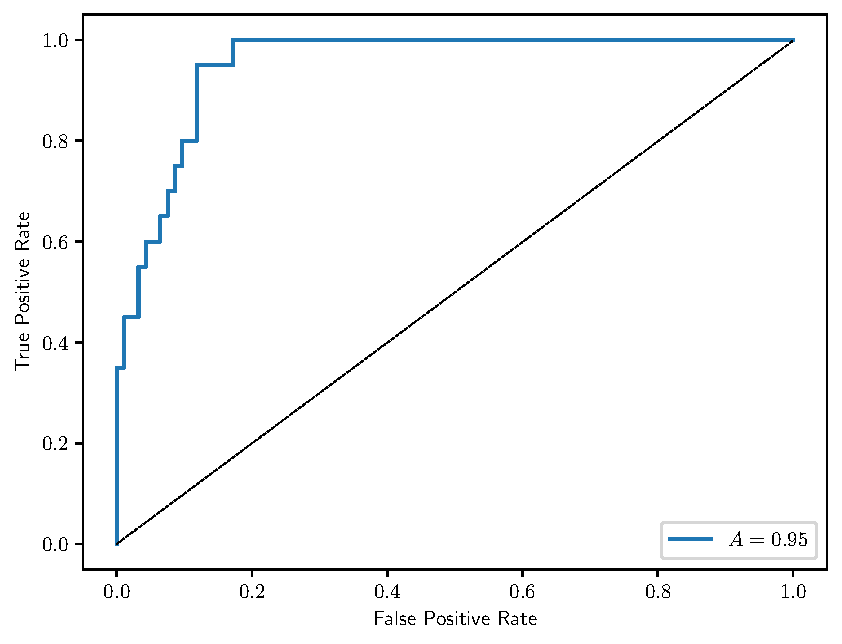
\includegraphics[width=\textwidth]{figs/2-0.9-roc.pdf}
    \caption{ROC curve.}
  \end{subfigure}
  \caption{Learning curves for $\mathcal{L}=[2]$ network with $\eta=0.9$ (2nd
    best).}
  \label{fig:NN-2best}
\end{figure*}

\begin{figure*}
  \centering
  \begin{subfigure}[b]{0.32\textwidth}
    \centering 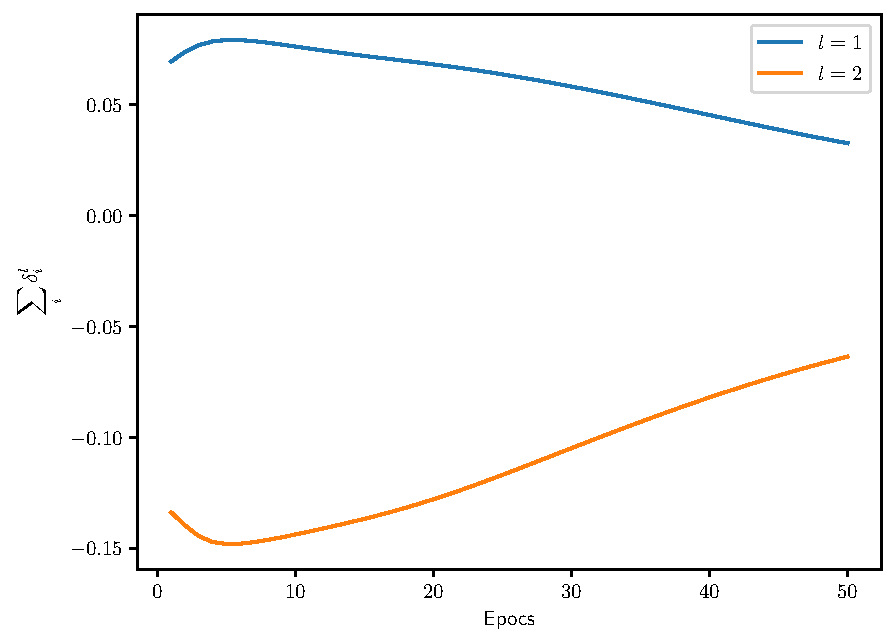
\includegraphics[width=\textwidth]{figs/3-0.9-gradients.pdf}
    \caption{Gradients for each layer.}
  \end{subfigure}
  \begin{subfigure}[b]{0.32\textwidth}
    \centering 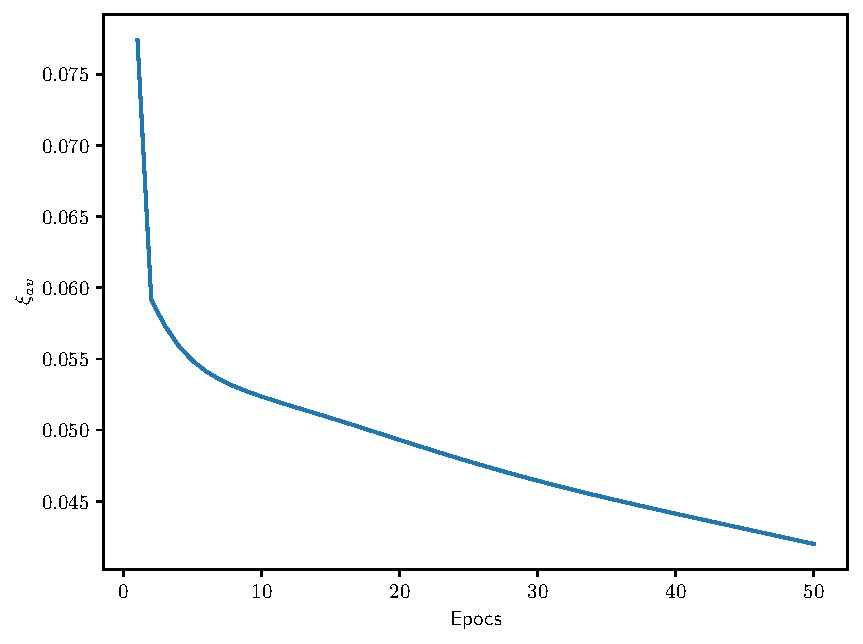
\includegraphics[width=\textwidth]{figs/3-0.9-error.pdf}
    \caption{Average error energy per epoch.}
  \end{subfigure}
  \begin{subfigure}[b]{0.32\textwidth}
    \centering 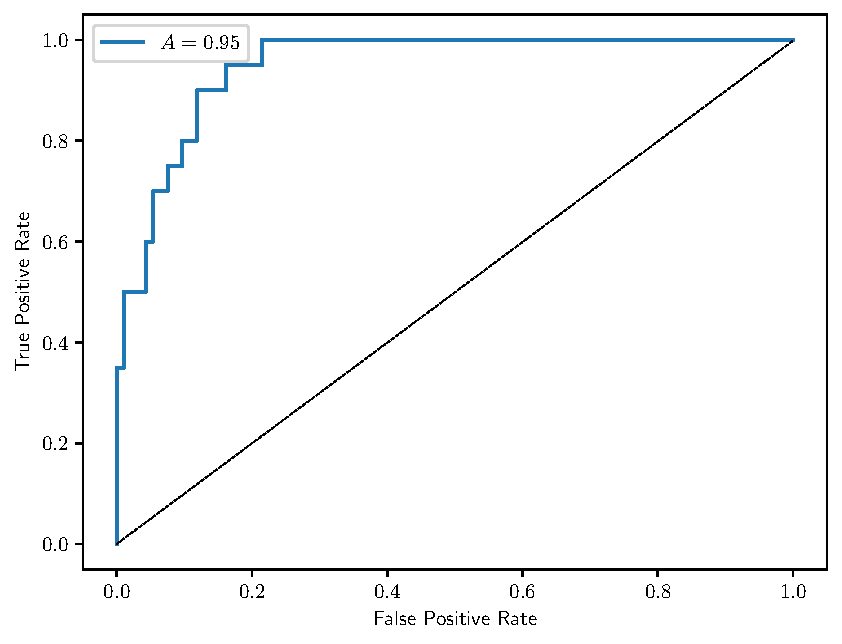
\includegraphics[width=\textwidth]{figs/3-0.9-roc.pdf}
    \caption{ROC curve.}
  \end{subfigure}
  \caption{Learning curves for $\mathcal{L}=[3]$ network with $\eta=0.9$
    (best).}
  \label{fig:NN-best}
\end{figure*}

\begin{table}
  \centering
  \caption{Performance scores for $\mathcal{L}=[1,2,3]$ and $\eta=0.9$.}
  \label{tab:L123}
  \begin{tabular}{ccc}
    \hline
    \textbf{Set} & \textbf{Sensitivity} & \textbf{Specificity} \\ \hline
    Training & 0 & 1 \\
    Testing & 0 & 1 \\
    Validation & 0 & 1 \\ \hline
  \end{tabular}
\end{table}

\begin{table}
  \centering
  \caption{Performance scores for $\mathcal{L}=[2]$ and $\eta=0.9$.}
  \label{tab:L2}
  \begin{tabular}{ccc}
    \hline
    \textbf{Set} & \textbf{Sensitivity} & \textbf{Specificity} \\ \hline
    Training & $\times$ & 1 \\
    Testing & $\times$ & 1 \\
    Validation & $\times$ & 1 \\ \hline
  \end{tabular}
\end{table}

\begin{table}
  \centering
  \caption{Performance scores for $\mathcal{L}=[3]$ and $\eta=0.9$.}
  \label{tab:L3}
  \begin{tabular}{ccc}
    \hline
    \textbf{Set} & \textbf{Sensitivity} & \textbf{Specificity} \\ \hline
    Training & 0.5 & 1 \\
    Testing & $\times$ & 1 \\
    Validation & 1 & 1 \\ \hline
  \end{tabular}
\end{table}

\section{Conclusions}\label{sec:conc}
The results presented gave insight on how the two classes could be separated.
The authors are keen on the idea that these shattered points could be mapped
into a more intuitive interpretation of individuals requiring psychological
attention (class 0) and others that show apparent ``normal'' conditions (class
1). Note that this is pure speculation and would need confirmation by better
qualified personnel.

As for future work, the hypothesis and results here presented could be reviewed
by an expert, since this work is preliminary and the authors are no experts in
Mental Health. Additionally, a better review of sophisticated techniques for
visualizing learning machines could be done, since the 2-dimensional embedding
of the decision function (contours) was more of an heuristic approach proposed
by the authors and it could be somehow improved. Finally, the inclusion of more
metrics for evaluating the performance of the classifiers can be included as
well, since only the Sensitivity-Specificity was done.

\printbibliography

\newpage
\appendices

\section{Results for Embedded Data}\label{app:emb}
This section presents the same results above presented but for the data
embedded with the TSNE algorithm prior to training.

\subsection{Support Vector Machines}
The PAC learning, results using the same optimization-sensitivity methodology,
are presented in Fig. \ref{fig:error-SVM-emb}

\begin{figure}
    \centering
    \begin{subfigure}[b]{0.45\textwidth}
        \centering
        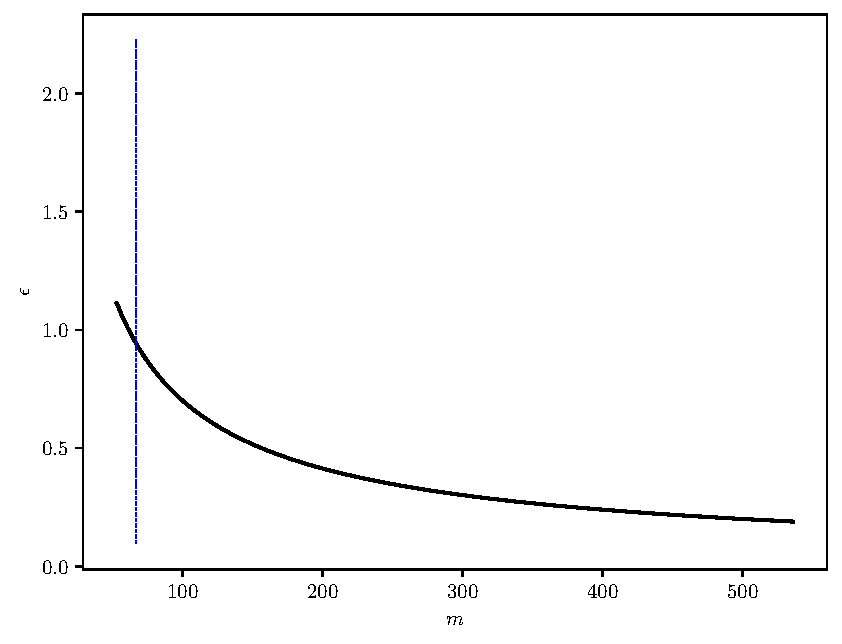
\includegraphics[width=\textwidth]{figs/svm-emb-linear-error.pdf}
        \caption{Linear SVM.}
    \end{subfigure}
    \begin{subfigure}[b]{0.45\textwidth}
        \centering
        \includegraphics[width=\textwidth]{figs/svm-emb-poly-error.pdf}
        \caption{Polynomial SVM}
    \end{subfigure}
    \caption{Estimated $\epsilon$ for different training set sizes.}
    \label{fig:error-SVM-emb}
\end{figure}

\begin{figure}
  \includegraphics[width=\columnwidth]{figs/svm-emb-linear-contour-0-1.pdf}
  \caption{Linear kernel SVM contour with real labels.}
\end{figure}

\begin{table}
\centering
\caption{Performance scores for linear SVM.}
\label{tab:linear_SVM_emb}
\begin{tabular}{ccc}
\hline
\textbf{Set} & \textbf{Sensitivity} & \textbf{Specificity} \\ \hline
Training & 0 & 1 \\
Testing & 0 & 1 \\
Validation & 0 & 1 \\ \hline
\end{tabular}
\end{table}

\begin{figure}
  \includegraphics[width=\columnwidth]{figs/svm-emb-poly-contour-0-1.pdf}
  \caption{Polynomial kernel SVM contour with real labels.}
\end{figure}

\begin{table}
\centering
\caption{Performance scores for polynomial SVM.}
\label{tab:poly_SVM_emb}
\begin{tabular}{ccc}
\hline
\textbf{Set} & \textbf{Sensitivity} & \textbf{Specificity} \\ \hline
Training & 0 & 1 \\
Testing & 0 & 1 \\
Validation & 0 & 1 \\ \hline
\end{tabular}
\end{table}

\begin{figure}
  \includegraphics[width=\columnwidth]{figs/svm-emb-rbf-contour-0-1.pdf}
  \caption{RBF kernel SVM contour with real labels.}
\end{figure}

\begin{table}
\centering
\caption{Performance scores for polynomial RBF.}
\label{tab:rbf_SVM_emb}
\begin{tabular}{ccc}
\hline
\textbf{Set} & \textbf{Sensitivity} & \textbf{Specificity} \\ \hline
Training & 0 & 1 \\
Testing & 0 & 1 \\
Validation & 0 & 1 \\ \hline
\end{tabular}
\end{table}

\subsection{Decision Tree}
The estimated value of $\epsilon$ for the given training dataset size, taking
$m=2$, a tree depth $k=5$ and a fixed $\delta=0.3$ is 0.5763.
\begin{figure}
    \includegraphics[width=\columnwidth]{figs/tree-emb-graph.pdf}
    \caption{Decision tree.}
\end{figure}

\begin{figure}
    \includegraphics[width=\columnwidth]{figs/tree-contour-0-1.pdf}
    \caption{Decision Tree contour with real labels.}
\end{figure}

\begin{table}
\centering
\caption{Performance scores for DT.}
\label{tab:DT_emb}
\begin{tabular}{ccc}
\hline
\textbf{Set} & \textbf{Sensitivity} & \textbf{Specificity} \\ \hline
Training & 1 & 1 \\
Testing & 0 & 1 \\
Validation & 0.63 & 0.94 \\ \hline
\end{tabular}
\end{table}

\subsection{Neural Networks}
\begin{figure*}
    \centering
    \begin{subfigure}[b]{0.32\textwidth}
        \centering
        \includegraphics[width=\textwidth]{figs/2-3-3-0.9-emb-gradients.pdf}
        \caption{Gradients for each layer.}
    \end{subfigure}
    \begin{subfigure}[b]{0.32\textwidth}
        \centering
        \includegraphics[width=\textwidth]{figs/2-3-3-0.9-emb-error.pdf}
        \caption{Average error energy per epoch.}
    \end{subfigure}
    \begin{subfigure}[b]{0.32\textwidth}
        \centering
        \includegraphics[width=\textwidth]{figs/2-3-3-0.9-emb-roc.pdf}
        \caption{ROC curve.}
    \end{subfigure}
    \caption{Learning curves for $\mathcal{L}=[2,3,3]$ network with $\eta=0.9$
    (worst).}
\end{figure*}

\begin{figure*}
    \centering
    \begin{subfigure}[b]{0.32\textwidth}
        \centering
        \includegraphics[width=\textwidth]{figs/3-0.5-emb-gradients.pdf}
        \caption{Gradients for each layer.}
    \end{subfigure}
    \begin{subfigure}[b]{0.32\textwidth}
        \centering
        \includegraphics[width=\textwidth]{figs/3-0.5-emb-error.pdf}
        \caption{Average error energy per epoch.}
    \end{subfigure}
    \begin{subfigure}[b]{0.32\textwidth}
        \centering
        \includegraphics[width=\textwidth]{figs/3-0.5-emb-roc.pdf}
        \caption{ROC curve.}
    \end{subfigure}
    \caption{Learning curves for $\mathcal{L}=[3]$ with $\eta=0.5$ network
    (2nd best).}
\end{figure*}

\begin{figure*}
    \centering
    \begin{subfigure}[b]{0.32\textwidth}
        \centering
        \includegraphics[width=\textwidth]{figs/2-0.2-emb-gradients.pdf}
        \caption{Gradients for each layer.}
    \end{subfigure}
    \begin{subfigure}[b]{0.32\textwidth}
        \centering
        \includegraphics[width=\textwidth]{figs/2-0.2-emb-error.pdf}
        \caption{Average error energy per epoch.}
    \end{subfigure}
    \begin{subfigure}[b]{0.32\textwidth}
        \centering
        \includegraphics[width=\textwidth]{figs/2-0.2-emb-roc.pdf}
        \caption{ROC curve.}
    \end{subfigure}
    \caption{Learning curves for $\mathcal{L}=[2]$ with $\eta=0.2$ network
    (best).}
\end{figure*}

\begin{table}
\centering
\caption{Performance scores for $\mathcal{L}=[2]$ and $\eta=0.2$.}
\label{tab:L2_emb}
\begin{tabular}{ccc}
\hline
\textbf{Set} & \textbf{Sensitivity} & \textbf{Specificity} \\ \hline
Training & $\times$ & 1 \\
Testing & $\times$ & 1 \\
Validation & $\times$ & 1 \\ \hline
\end{tabular}
\end{table}

\begin{table}
\centering
\caption{Performance scores for $\mathcal{L}=[3]$ and $\eta=0.5$.}
\label{tab:L3_emb}
\begin{tabular}{ccc}
\hline
\textbf{Set} & \textbf{Sensitivity} & \textbf{Specificity} \\ \hline
Training & $\times$ & 1 \\
Testing & $\times$ & 1 \\
Validation & $\times$ & 1 \\ \hline
\end{tabular}
\end{table}

\begin{table}
\centering
\caption{Performance scores for $\mathcal{L}=[2,3,3]$ and $\eta=0.9$.}
\label{tab:L233_emb}
\begin{tabular}{ccc}
\hline
\textbf{Set} & \textbf{Sensitivity} & \textbf{Specificity} \\ \hline
Training & 0 & 1 \\
Testing & 0 & 1 \\
Validation & 0 & 1 \\ \hline
\end{tabular}
\end{table}

\end{document}
